\section{Introduction}

\tikzstyle{block} = [draw, rectangle, minimum height=3em, minimum width=3em]
\tikzstyle{gain} = [draw, colorful, regular polygon, regular polygon sides=3, shape border rotate=30]

\subsection{Visual programming}
\begin{frame}{Simulink is visual programming language}
  \begin{columns}
  \begin{column}{0.5\textwidth}
  \small
    \begin{itemize}
    \item Visual programming allows users to create programs by manipulating program elements graphically rather than by specifying them textually.
    \item A visual representation of algorithms is more intuitive 
    \item Visual languages help in understanding and designing of systems by visualizing the flow of operations.
    \item Visual languages may be more accessible to people without informatics background. 
  \end{itemize}
  \end{column}
  \begin{column}{0.5\textwidth}
  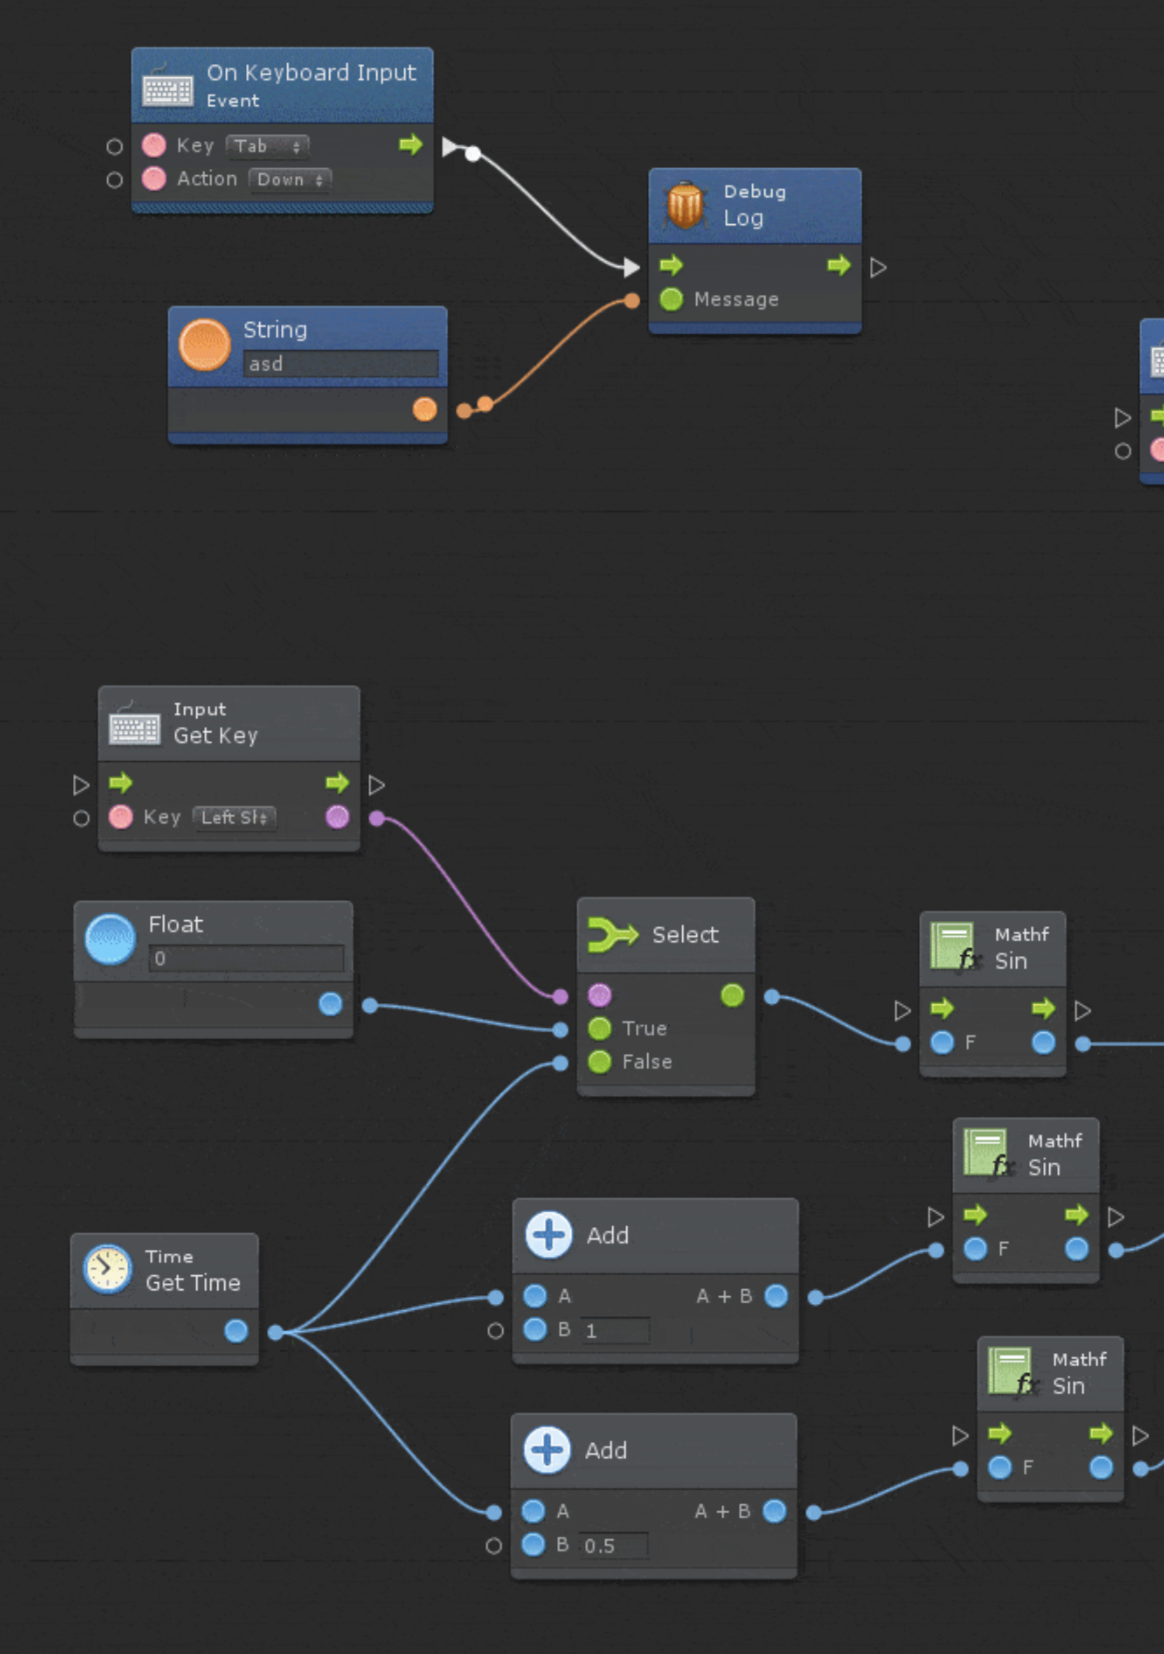
\includegraphics[scale = 0.2]{lesson_2/images/simulink_visual_programming.png}
  \end{column}
  \end{columns}
\end{frame}

\begin{frame}{Examples of visual programming languages}
\small
\begin{itemize}
    \item \textbf{Simulink (MathWorks)}: A graphical programming environment by for simulating and analyzing multidomain systems. It offers a drag-and-drop interface with block libraries for system and algorithm modeling, widely used in engineering and aerospace for design and simulation.
    
    \item \textbf{LabVIEW (National Instruments)}:
    A graphical platform for data acquisition, instrument control, and automation. LabVIEW uses a block diagram approach for developing measurement and control systems, suitable for engineers and scientists needing to implement complex systems without deep programming knowledge.

    \item \textbf{Scratch (MIT Media Lab)}:
    A block-based visual programming language designed for children and beginners. It allows users to create animations, games, and stories through an intuitive interface, promoting logical thinking and creativity in education.
\end{itemize}
\end{frame}


\begin{frame}{How Simulink Works}
\small
  \begin{itemize}
    \item Users assemble \textbf{block diagrams} by selecting \textbf{blocks} from a library and connecting them with \textbf{lines} that represent data flow. 
    \pause
    \item At the start of simulation, model specifies the initial states and outputs of the system to be simulated.
    \pause
    \item Simulation runs in loop: At each time step, Simulink computes the new values for the system inputs, states and outputs and updates the model to reflect the computed values. (Think of \textit{for loop} iterations we did earlier)  
    \pause
    \item At the end of the simulation, the model reflects the final values of the systems inputs, states and outputs
    \pause
    \item  Simulink provides data logging and display functionality to show data during the simulation.
    \item Close integration with MATLAB enables creating Simulink models by coding in Matlab, transfer data to and from Matlab and many other functions.
\end{itemize}
\end{frame}

\begin{frame}{Applications of Simulink}
  \begin{itemize}
    \item \textbf{Engineering}: Used  in control systems, signal processing, communications, and robotics,
    \item \textbf{Automotive}:  in the design and test of control systems in vehicles, including engine management systems, advanced driver-assistance systems (ADAS), and autonomous driving technologies.
    \item \textbf{Aerospace}: designing flight control systems and navigation systems,
    \item \textbf{Energy Systems}: In the energy sector, Simulink supports the development of renewable energy systems, batteries, power electronics, and smart grid technologies.
    \item \textbf{Academia}: 
    \begin{itemize}
        \item tool in the teaching 
        \item modeling tool for many applications, including all topics we discuss in this course.
    \end{itemize}
  \end{itemize}
\end{frame}

\begin{frame}{Task}
    \Large
    \begin{enumerate}
        \item Find a job offering for position that requires knowledge of Simulink --- In English or other languages you know
        \item Find one academic peer-reviewed research article that uses Simulink. 
    \end{enumerate}
     
\end{frame}



\begin{frame}{Libraries offer functionality for various applications}

  \begin{itemize}
    \item \textbf{Simulink Standard Library:} Includes basic blocks for mathematical operations, logic, signal routing, and more. Essential for any model.
    \item \textbf{Simscape:} For physical modeling in domains such as mechanics, electrical, and fluids. Useful for simulating real-world system: Bateries, Electrical systems, Fluid, Mechanical applicatiosn
    \item \textbf{Stateflow:} Adds state machines and flow charts to Simulink models. Ideal for decision logic, mode scheduling, and event handling.
    \item \textbf{Code generation}: Generate C Code from Simulink models for deployment in a wide variety of applications
    \item \textbf{Control System Toolbox:} Offers blocks for designing and simulating control system, for models requiring feedback mechanisms.
  \end{itemize}
  

\end{frame}
\begin{frame}{Task}
    \begin{center}
    \Large
    \begin{itemize}
        \item Explores libraries at mathworks.com/products.
        \item Find one concrete example that you find interring.
    \end{itemize}
\end{center}
\end{frame}

\begin{frame}{Basic blocks: Integrator}
\begin{itemize}
    \item The Integrator block in Simulink performs the mathematical integration of an input signal over time.
    \item  In modeling populations, an integrator is used to simulate the cumulative effect of birth and death rates over time on a population's size.
    \item The \textbf{input} is a rate of change $\frac{dP}{dt}$ (here as the net growth rate of a population
    \item The \textbf{output} is integrator provides the total population $P$ at given time
\end{itemize}
\vfill

\begin{center}
    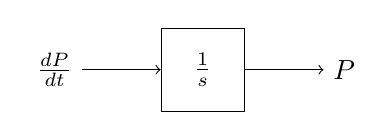
\begin{tikzpicture}
    % Block
    \node[block] (block1) {$\frac{1}{s}$};
    % Input
    \draw[<-] (block1.west) -- ++(-1,0) node[left] {$\frac{dP}{dt}$};
    % Output
    \draw[->] (block1.east) -- ++(1,0) node[right] {$P$};
\end{tikzpicture}
\end{center}
\end{frame}


\begin{frame}{Constant}
\begin{itemize}
    \item \textbf{Constants} in simulations represent fixed values that do not change over time.
    \item In population modeling, constants are essential for defining baseline conditions such as carrying capacity, initial population value or intrinsic growth rate
\end{itemize}
\vfill

\begin{center}
    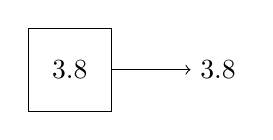
\begin{tikzpicture}[block/.style={draw, rectangle, minimum height=3em, minimum width=3em}]
    % Block
    \node[block] (block1) {$3.8$};
    % Output
    \draw[->] (block1.east) -- ++(1,0) node[right] {$3.8$};
\end{tikzpicture}
\end{center}
\end{frame}
\usetikzlibrary{positioning, shapes.geometric}

\begin{frame}{Other commons blocks: Products, Sum, and Gain}
\small
\begin{itemize}
    \item \textbf{Product Block}: Multiplies input signals. Used to represent interactions or dependencies between variables.
    \item \textbf{Sum Block}: Adds or subtracts input signals. Ideal for modeling net changes in a system, such as total population growth.
    \item \textbf{Gain Block}: Scales an input signal by a constant factor. Represents proportional relationships or amplification factors.
\end{itemize}
\vfill
\begin{center}
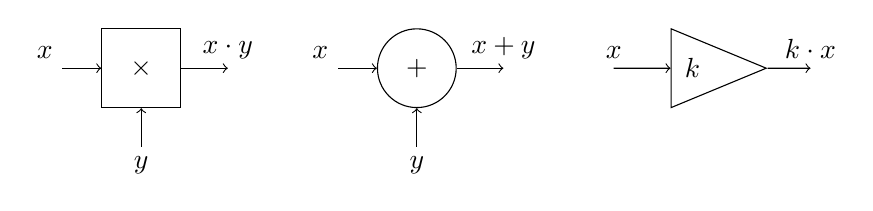
\begin{tikzpicture}[auto, node distance=2cm]
  % Product Block
    \node[draw, rectangle, minimum size=1cm] (product) at (0,0) {$\times$};
    \draw[<-] (product) -- ++(-1,0) node[above left] {$x$};
    \draw[<-] (product) -- ++(0,-1) node[below] {$y$};
    \draw[->] (product) -- ++(1.1,0) node[above] {$x \cdot y$};

    % Sum Block
    \node[draw, circle, minimum size=1cm] (sum) at (3.5,0) {+};
    \draw[<-] (sum) -- ++(-1,0) node[above left] {$x$};
    \draw[<-] (sum) -- ++(0,-1) node[below] {$y$};
    \draw[->] (sum) -- ++(1.1,0) node[above] {$x + y$};
    
    % Gain Block
    \node[draw, isosceles triangle, shape border rotate=0, minimum size=1cm] (gain) at (7,0) {$k$};
    \draw[<-] (gain) -- ++(-1,0) node[above] {$x$};
    \draw[->] (gain) -- ++(1.5,0) node[above] {$k \cdot x$};
\end{tikzpicture}

\end{center}
\end{frame}

\subsection{First simulations}
\begin{frame}{First simulation}
In this part you will learn how to
    \begin{itemize}
        \item Assemble your first model using library blocks
        \item Run a simulation
        \item Adjust simulation and display settings
    \end{itemize}
\vfill
\pause
We will start with a simple program that generates and displays a sine wave.  
\end{frame}
\begin{frame}{Open Simulink environment}
    \hspace*{-11mm}
    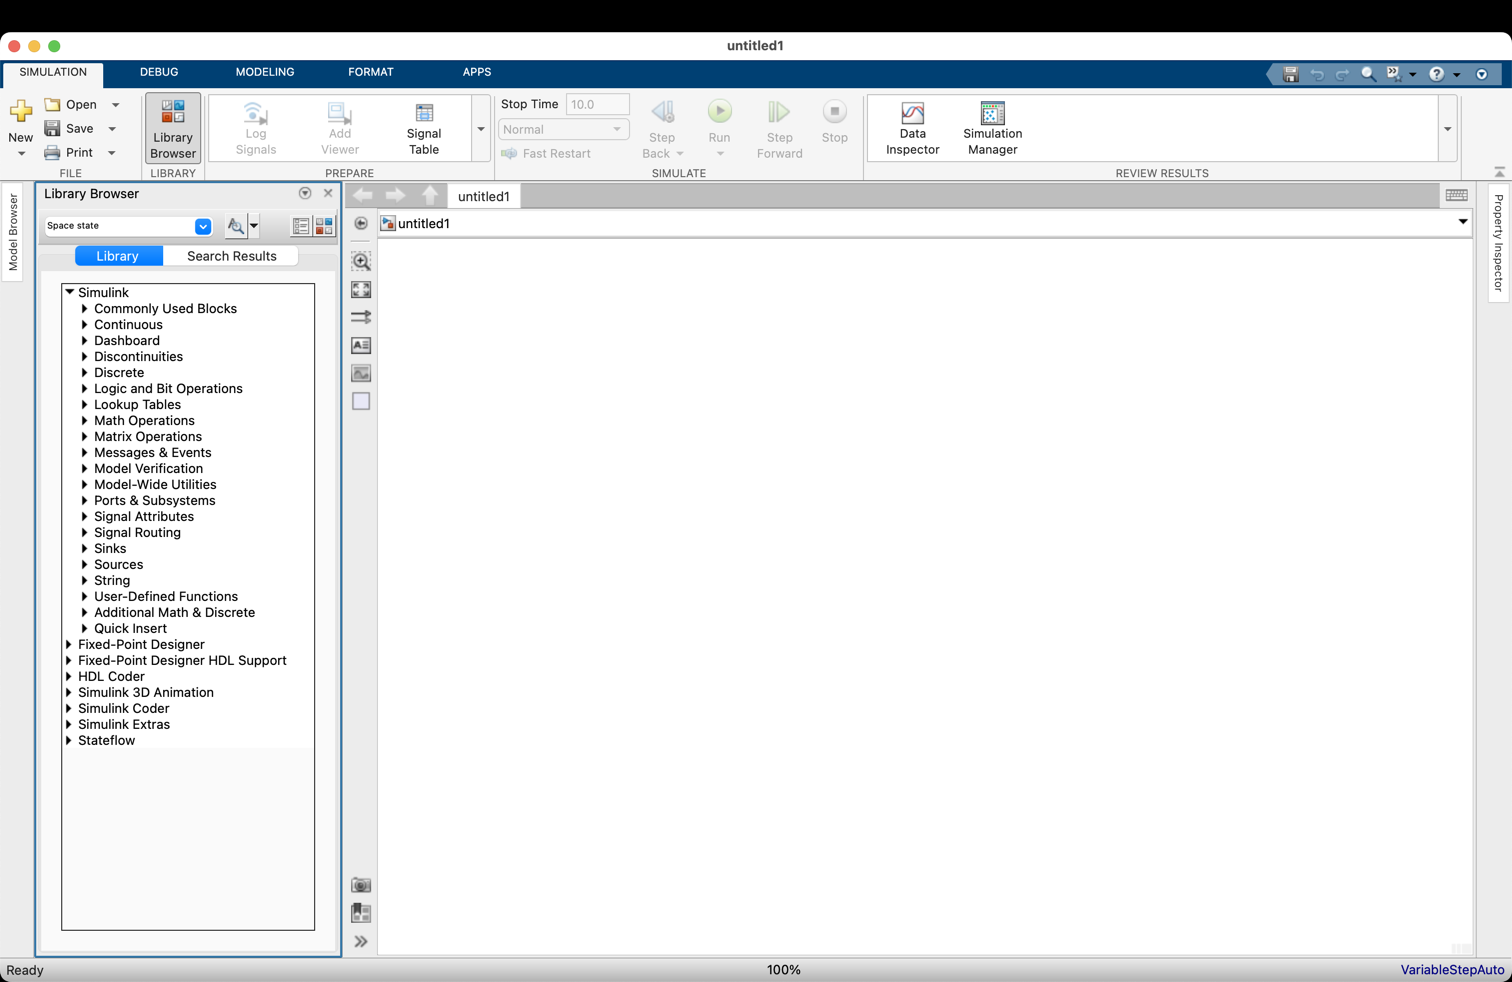
\includegraphics[width=\paperwidth]{lesson_2/images/simulink_screen_01.png}
\end{frame}

\begin{frame}{Drag a \textit{Sine wave} block from the library}
    \hspace*{-11mm}
    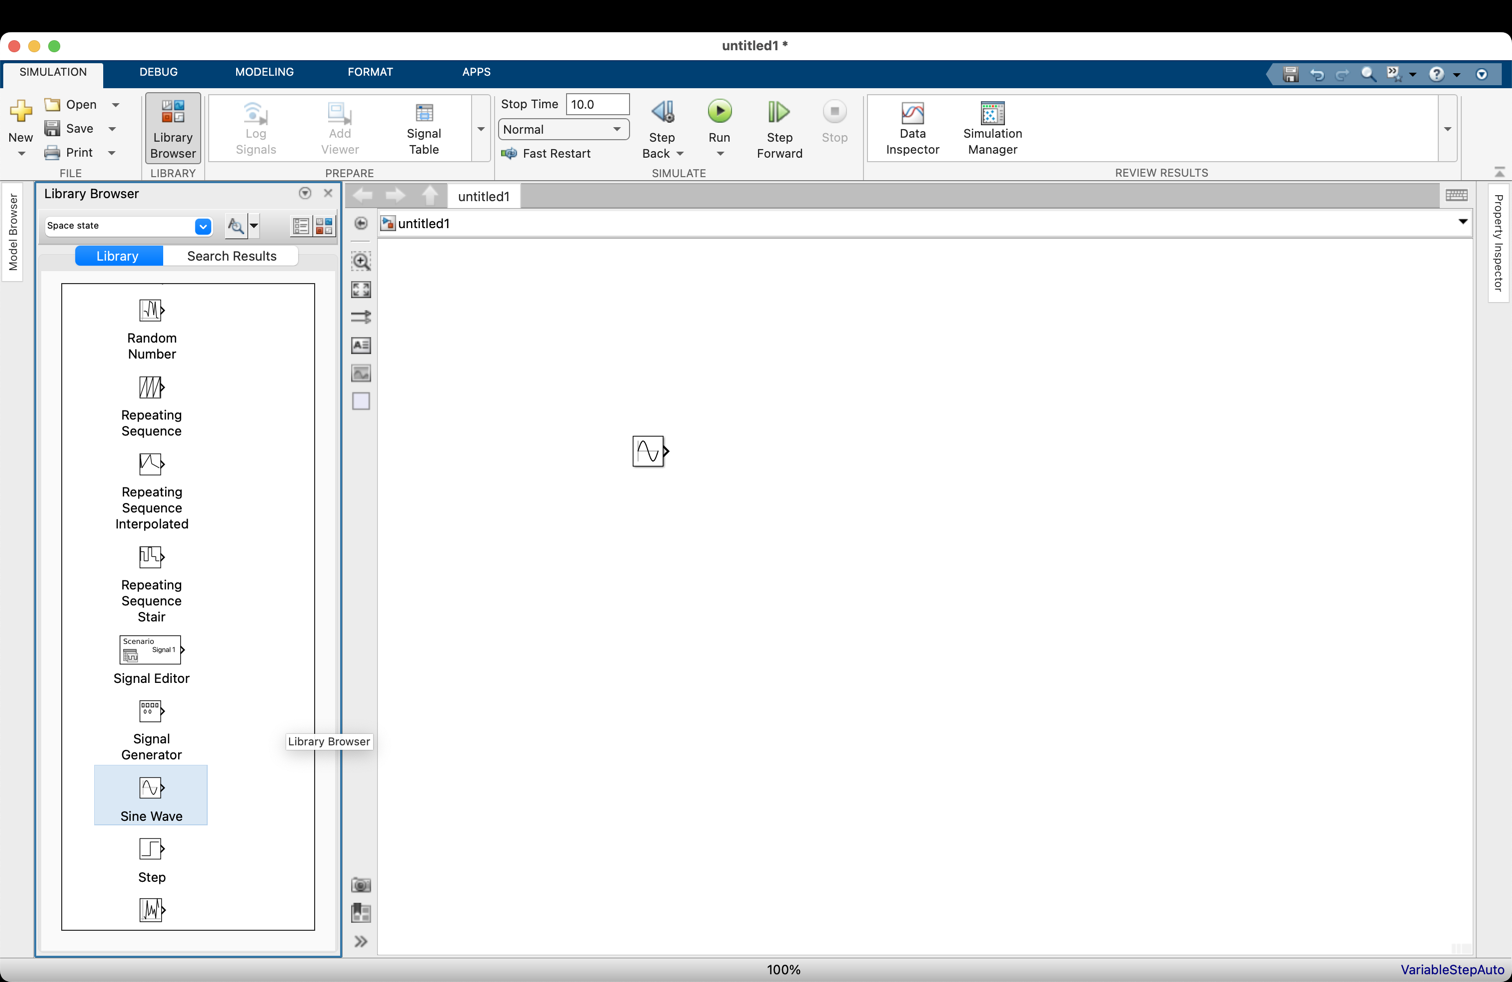
\includegraphics[width=\paperwidth]{lesson_2/images/simulink_screen_02.png}
\end{frame}
  
\begin{frame}{ Add \textit{Scope} and conncect blocs}
    \hspace*{-11mm}
    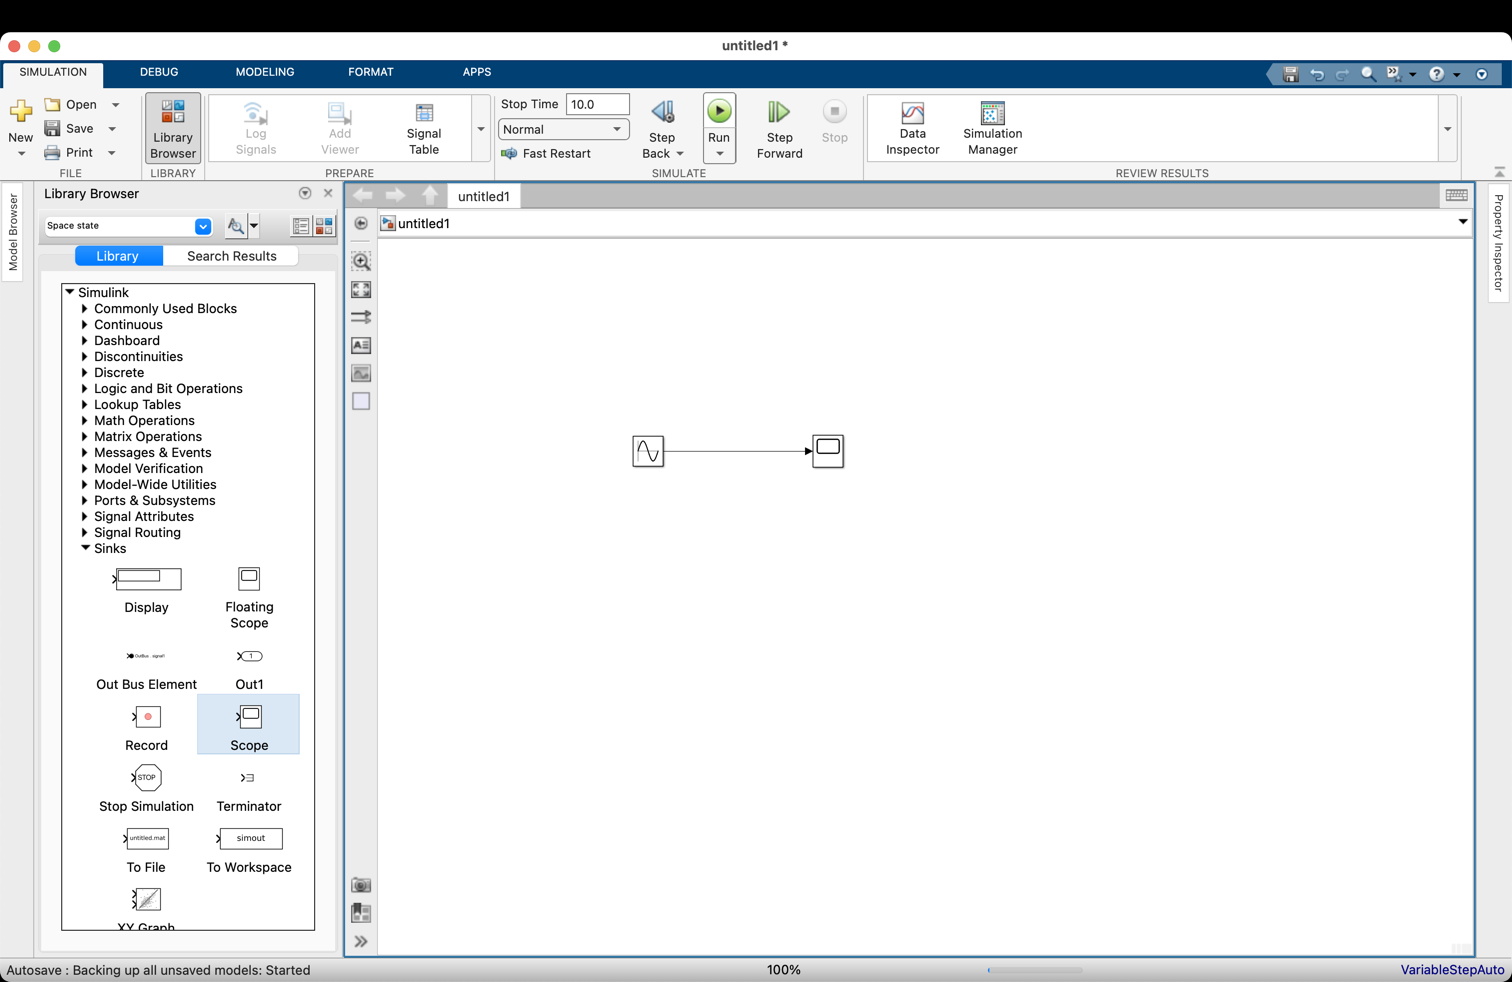
\includegraphics[width=\paperwidth]{lesson_2/images/simulink_screen_04.png}
\end{frame}
  
\begin{frame}{Run your first simulation}
    \hspace*{-11mm}
    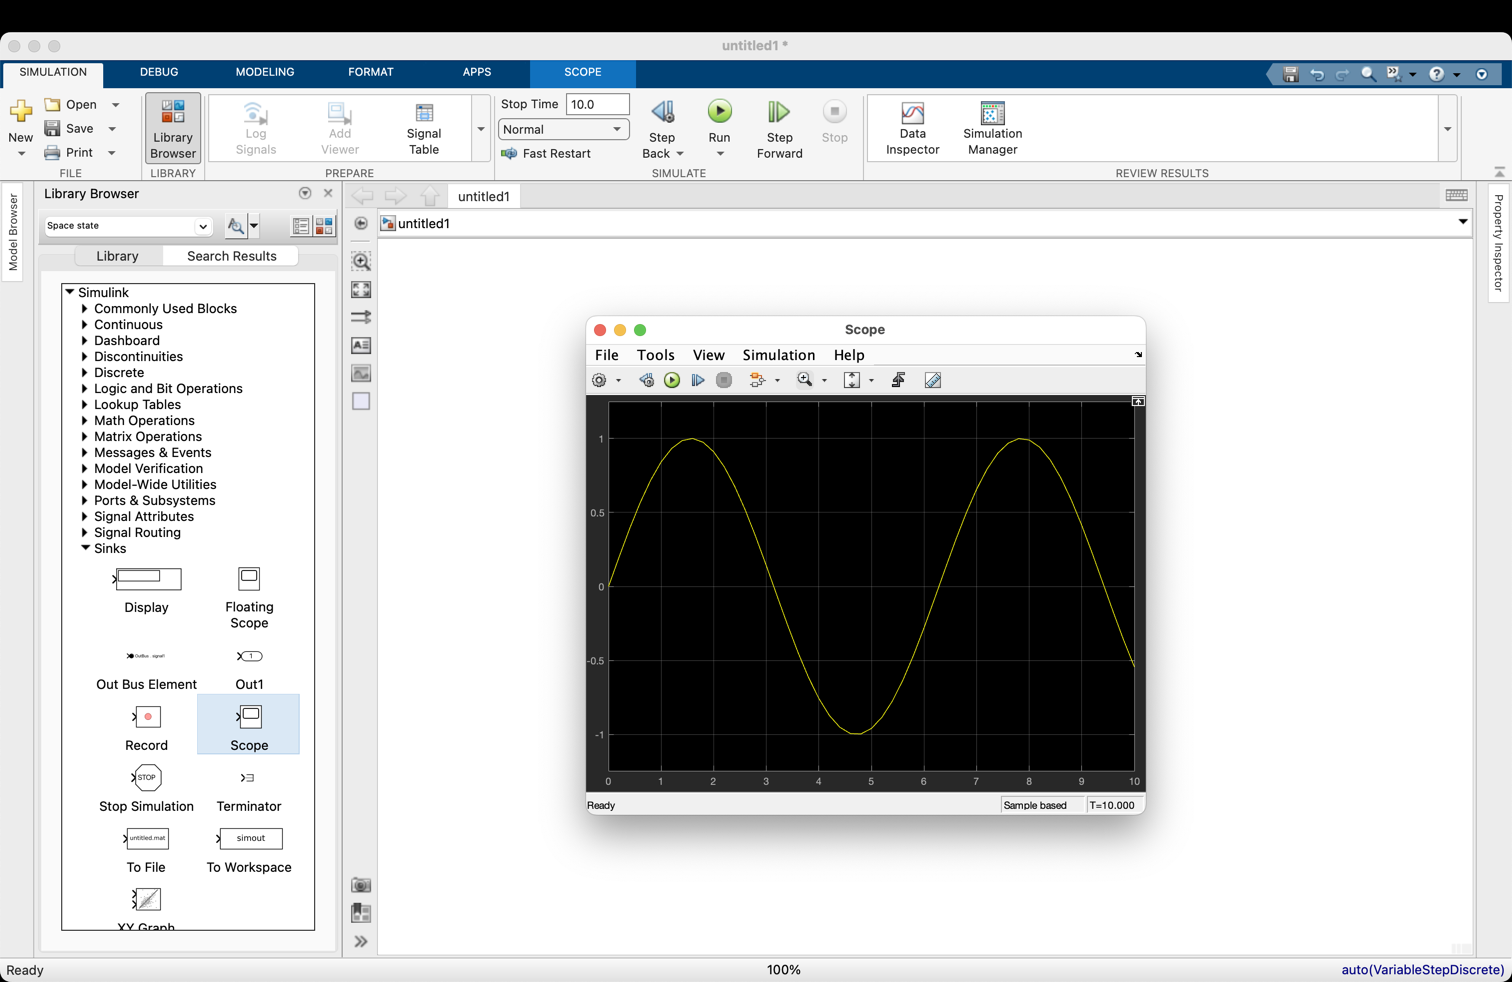
\includegraphics[width=\paperwidth]{lesson_2/images/simulink_screen_05.png}
\end{frame}

\subsection{Adjustment of simulation settings}
\begin{frame}{Simulate for longer time}
\Large
\begin{center}
    We now want to run the same simulation for longer time.\\
    \vfill
    \pause
    Adjust \textit{Stop time} to 100 and run again.
\end{center}
\end{frame}

\begin{frame}{Adjust \textit{Stop time} to 100 and run the simulation again.}
    \hspace*{-11mm}
    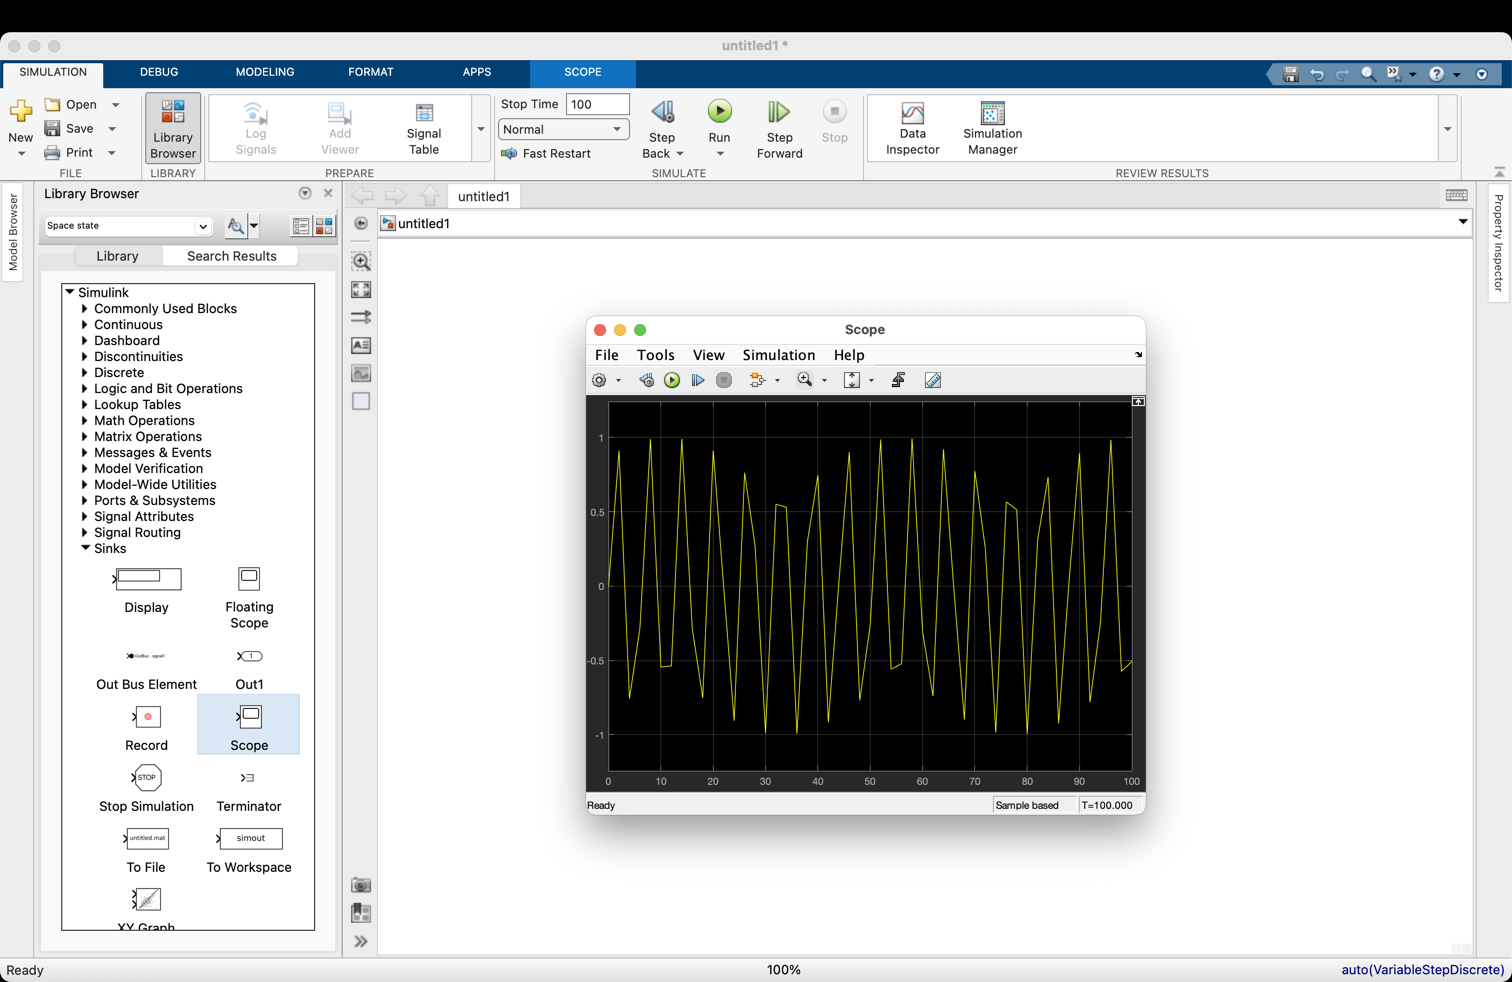
\includegraphics[width=\paperwidth]{lesson_2/images/simulink_screen_07.png}
\end{frame}

\begin{frame}{Problem with distotion}
\Large
\begin{center}
    Resulting wave looks incorrect --- Can you guess Why?.\\
    \pause
    \vfill
    The problem is distortion due to insufficient sampling frequency.\\
    \pause
    \vfill
    Low sampling frequency will affect our modeling. We need to adjust Model settings. 
\end{center}
\end{frame}


\begin{frame}{Select \textit{Modeling} and  \textit{Model Settings} }
    \hspace*{-11mm}
    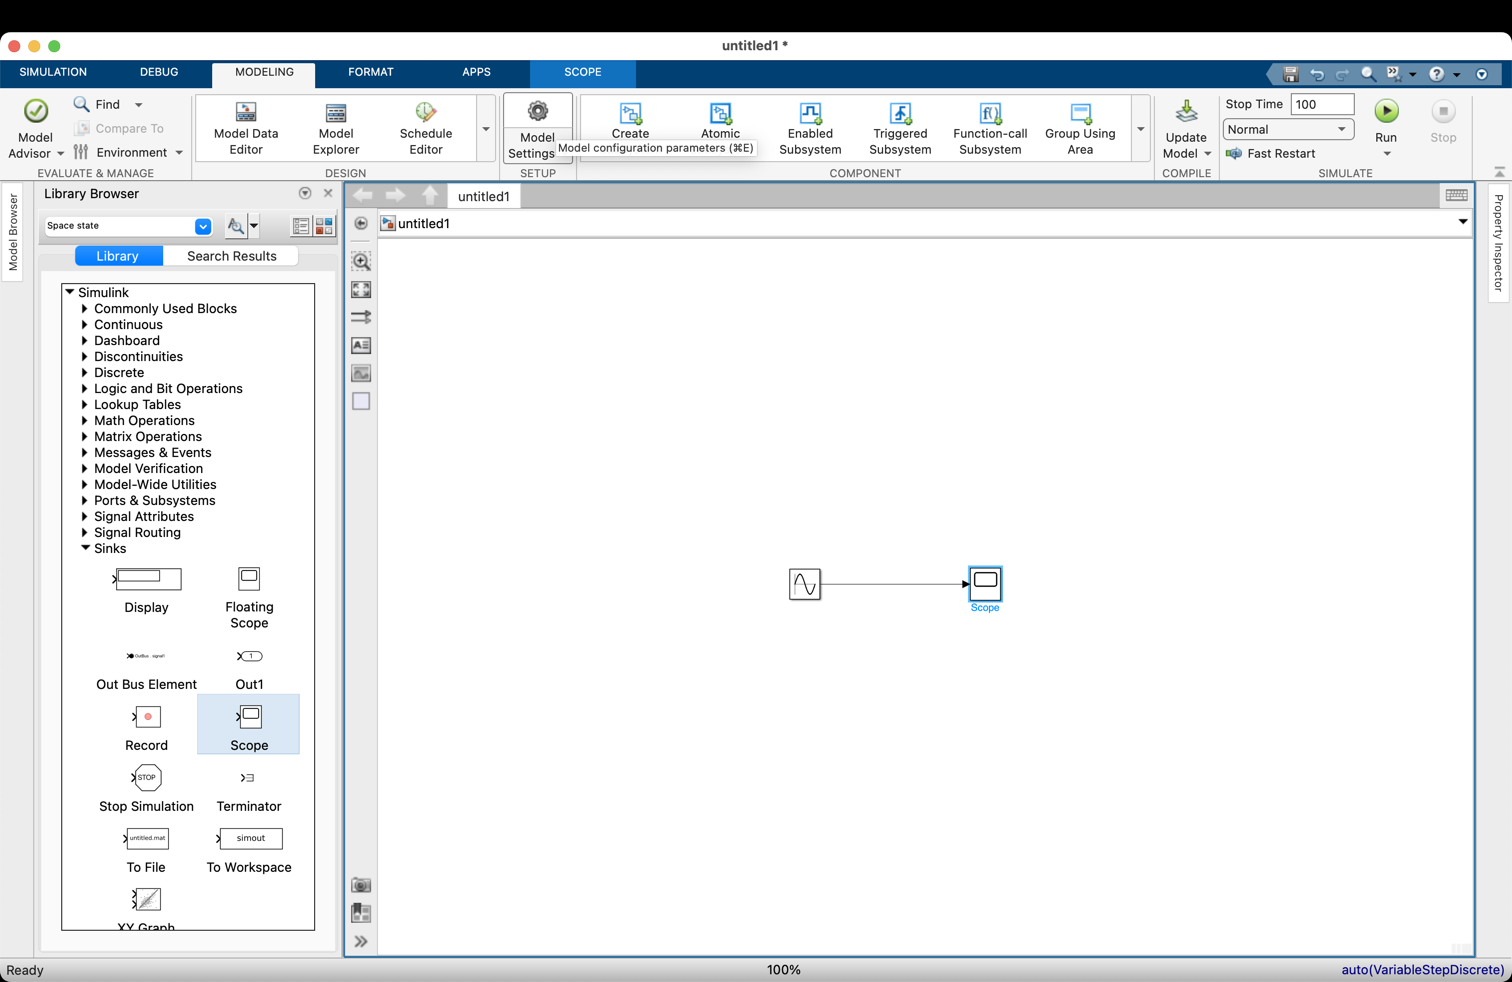
\includegraphics[width=\paperwidth]{lesson_2/images/simulink_screen_08.png}
\end{frame}

\begin{frame}{In \textit{Solver} menu select \textit{Fixed-step} type}
    \hspace*{-11mm}
    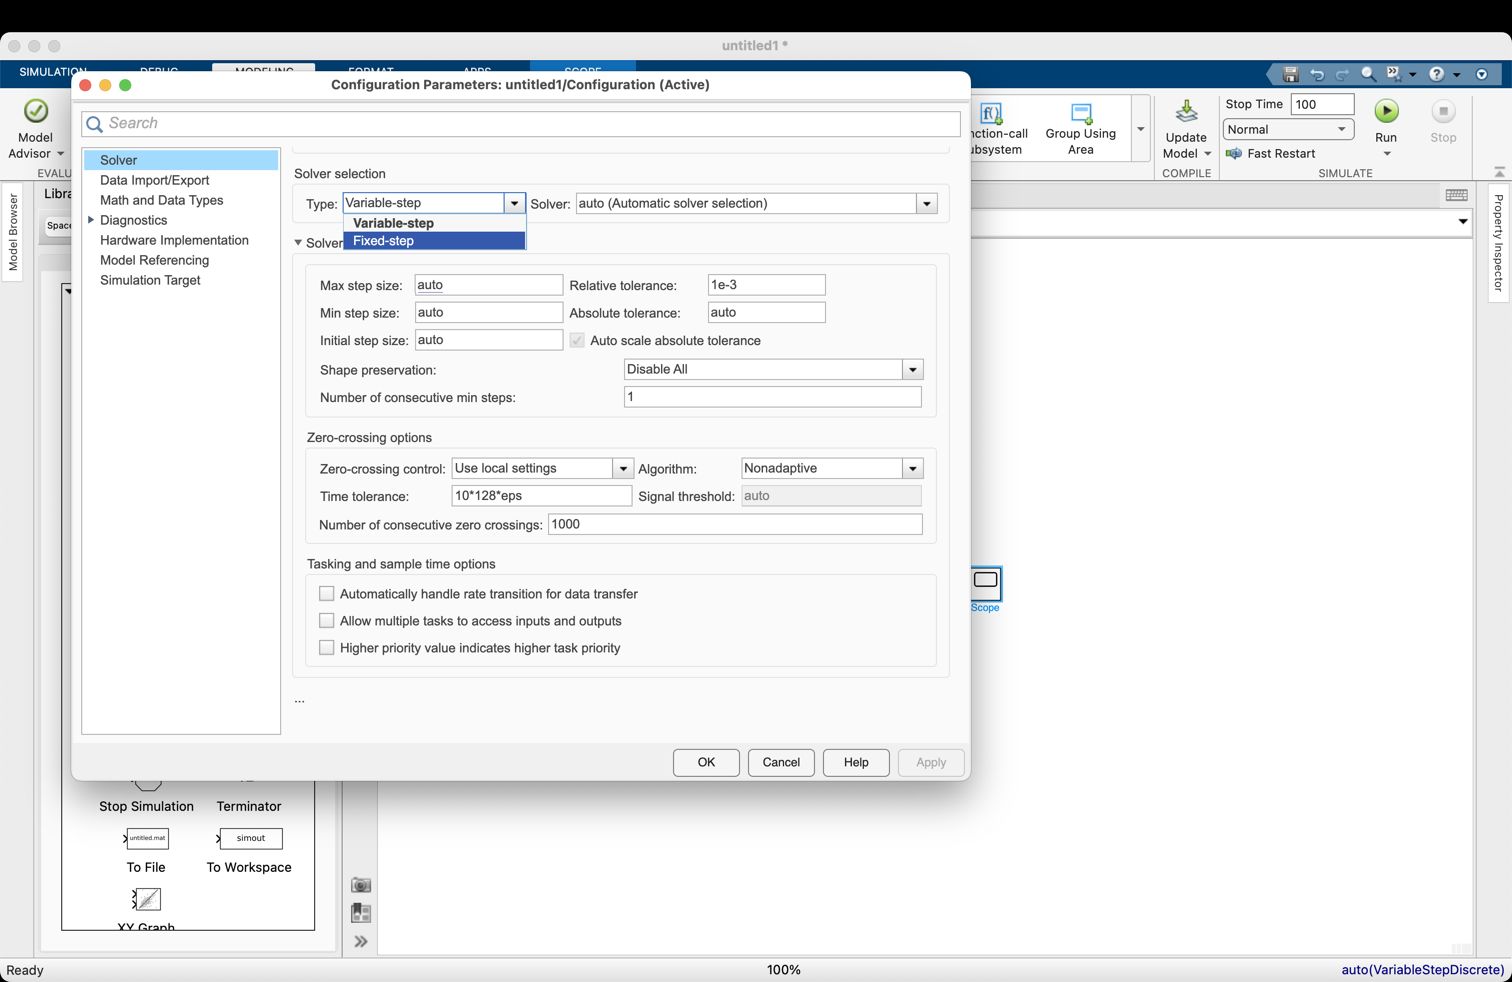
\includegraphics[width=\paperwidth]{lesson_2/images/simulink_screen_09.png}
\end{frame}

\begin{frame}{Adjust \textit{Fixed step} size to 0.1}
    \hspace*{-11mm}
    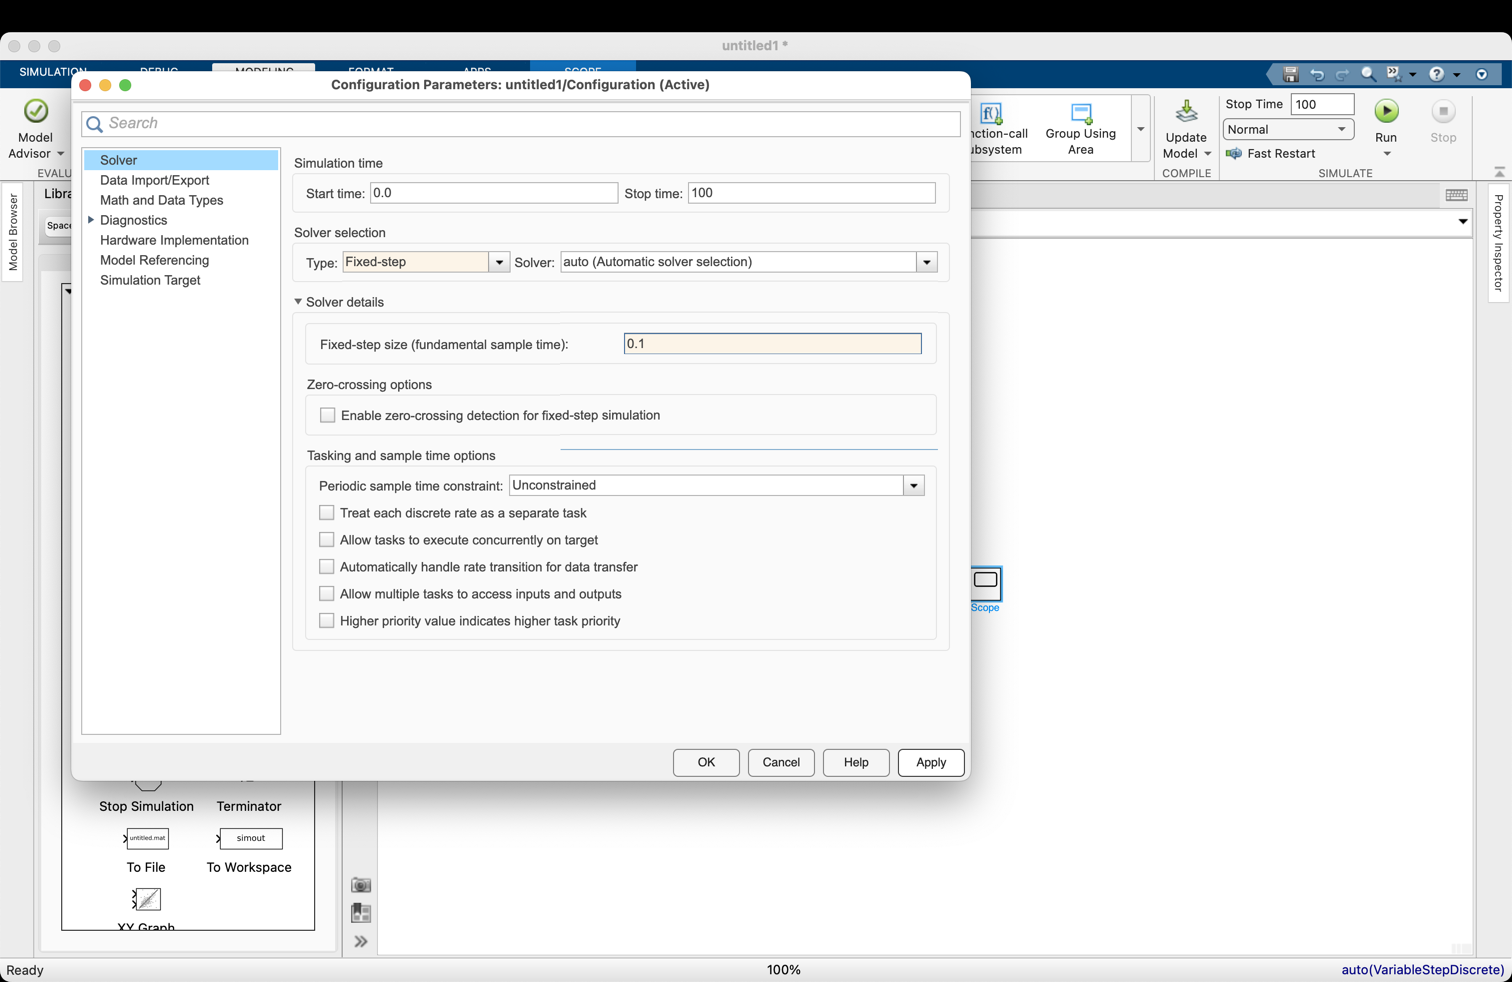
\includegraphics[width=\paperwidth]{lesson_2/images/simulink_screen_10.png}
\end{frame}

\begin{frame}{The curve should look correctly now.}
    \hspace*{-11mm}
    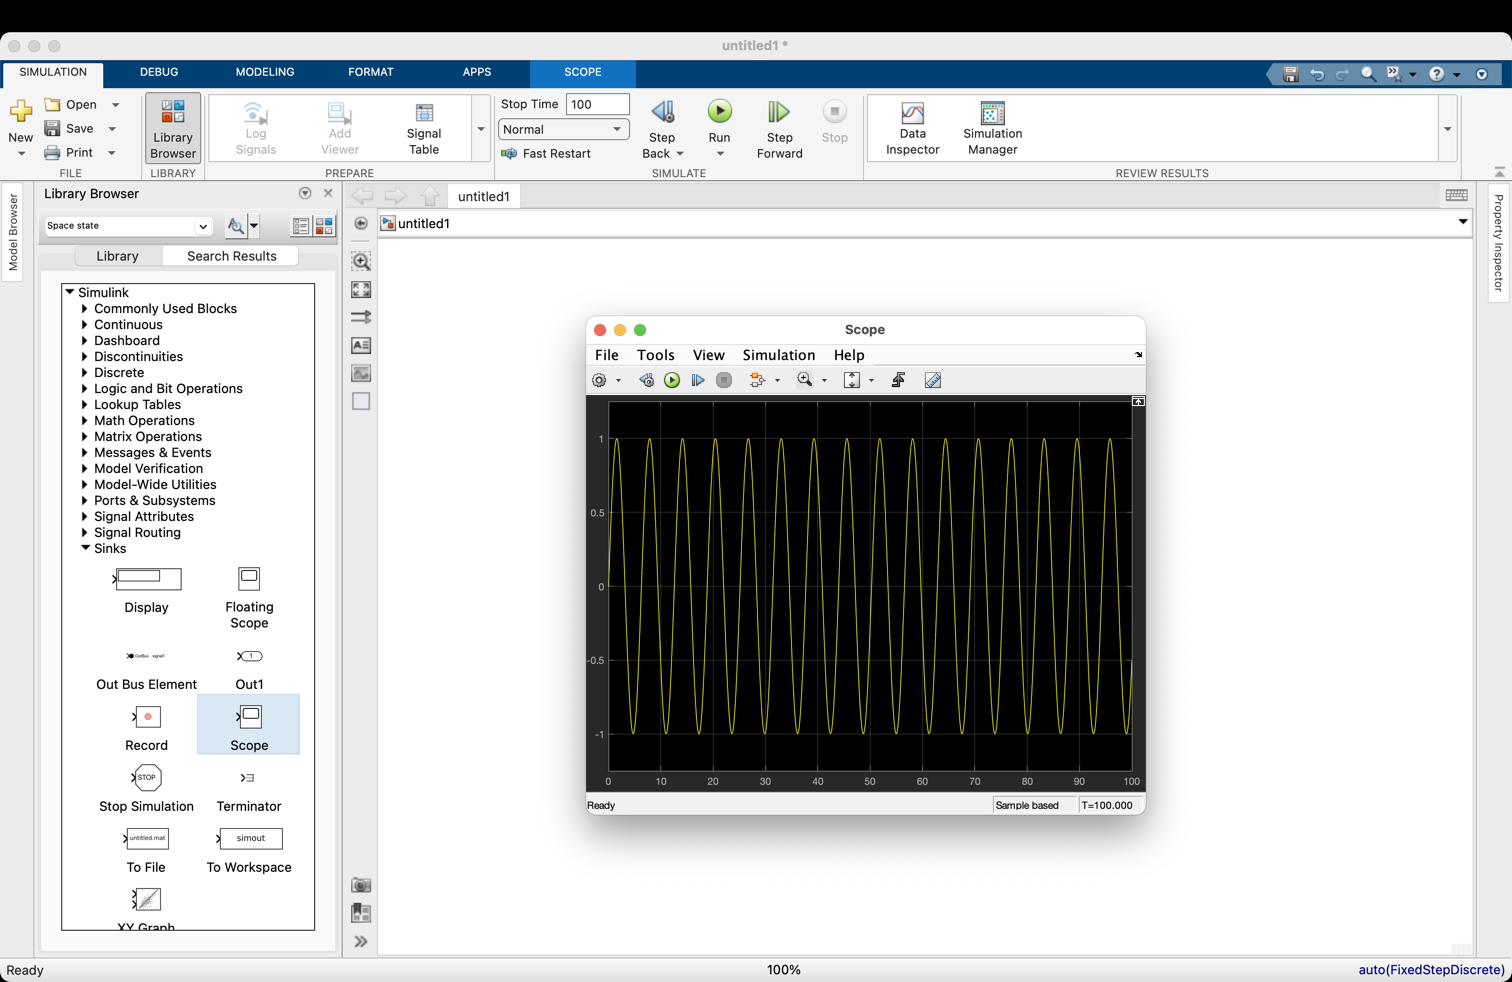
\includegraphics[width=\paperwidth]{lesson_2/images/simulink_screen_12.png}
\end{frame}

\subsection{Adjustment of simulation settings}
\begin{frame}{Simulate for longer time}
\Large
\begin{center}
We will now build a Malthusian model. 
\end{center}
\end{frame}


\begin{frame}{The core of the model is an integrator}
    \hspace*{-11mm}
    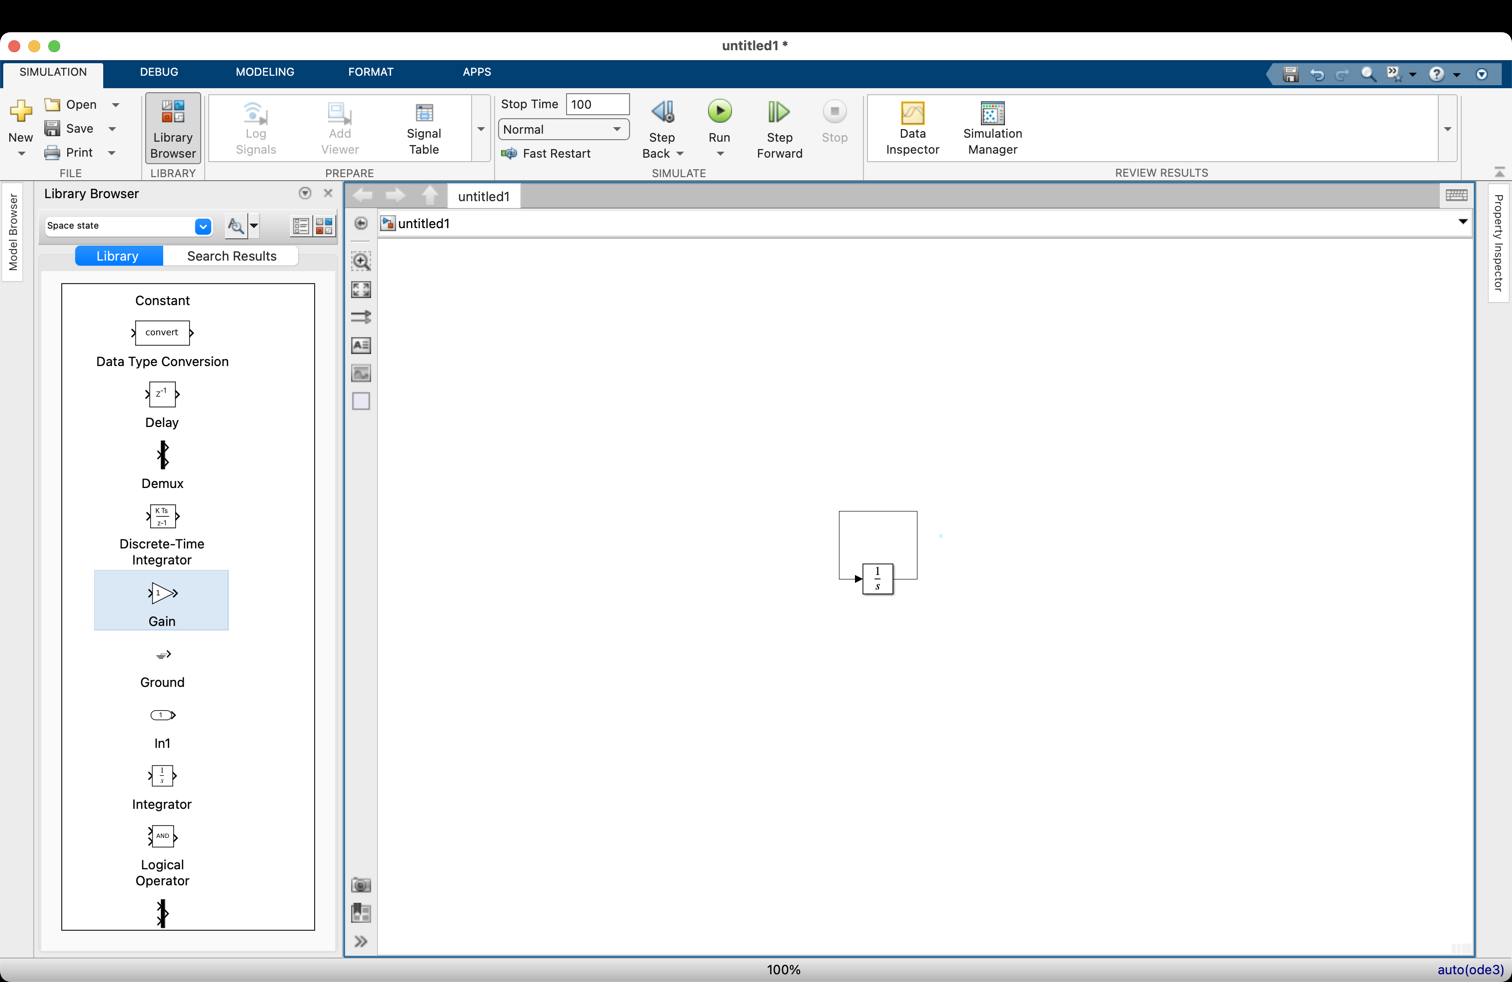
\includegraphics[width=\paperwidth]{lesson_2/images/simulink_screen_18.png}
\end{frame}

\begin{frame}{The core of the model is an integrator}
    \hspace*{-11mm}
    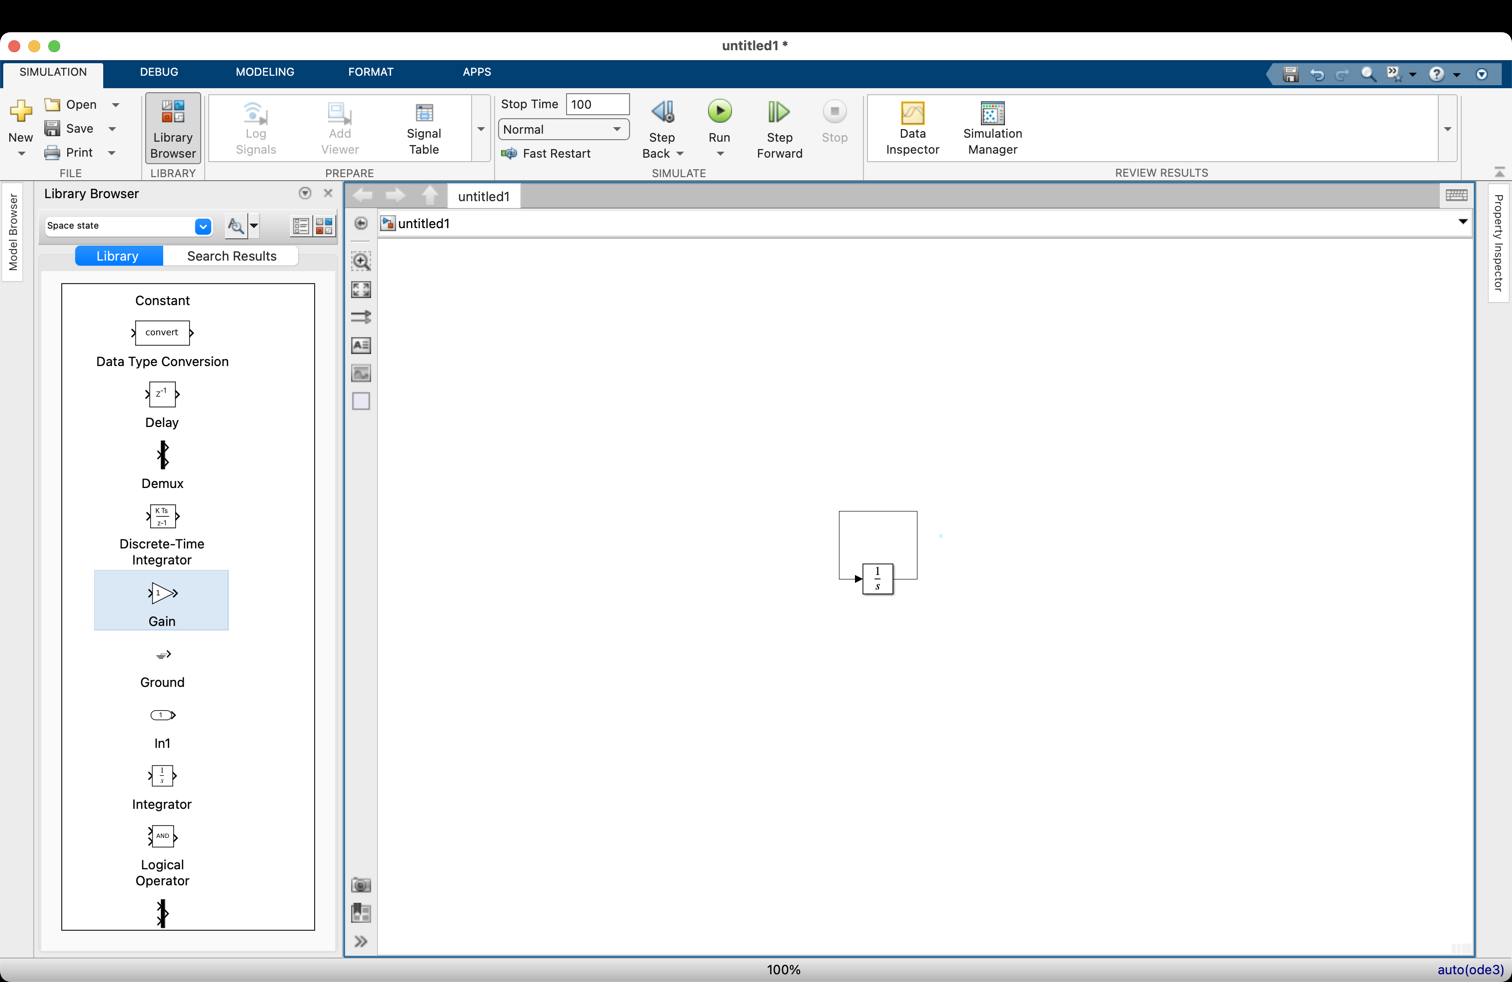
\includegraphics[width=\paperwidth]{lesson_2/images/simulink_screen_18.png}
\end{frame}

\begin{frame}{Gain element adjust magnitude of the signal.}
    \hspace*{-11mm}
    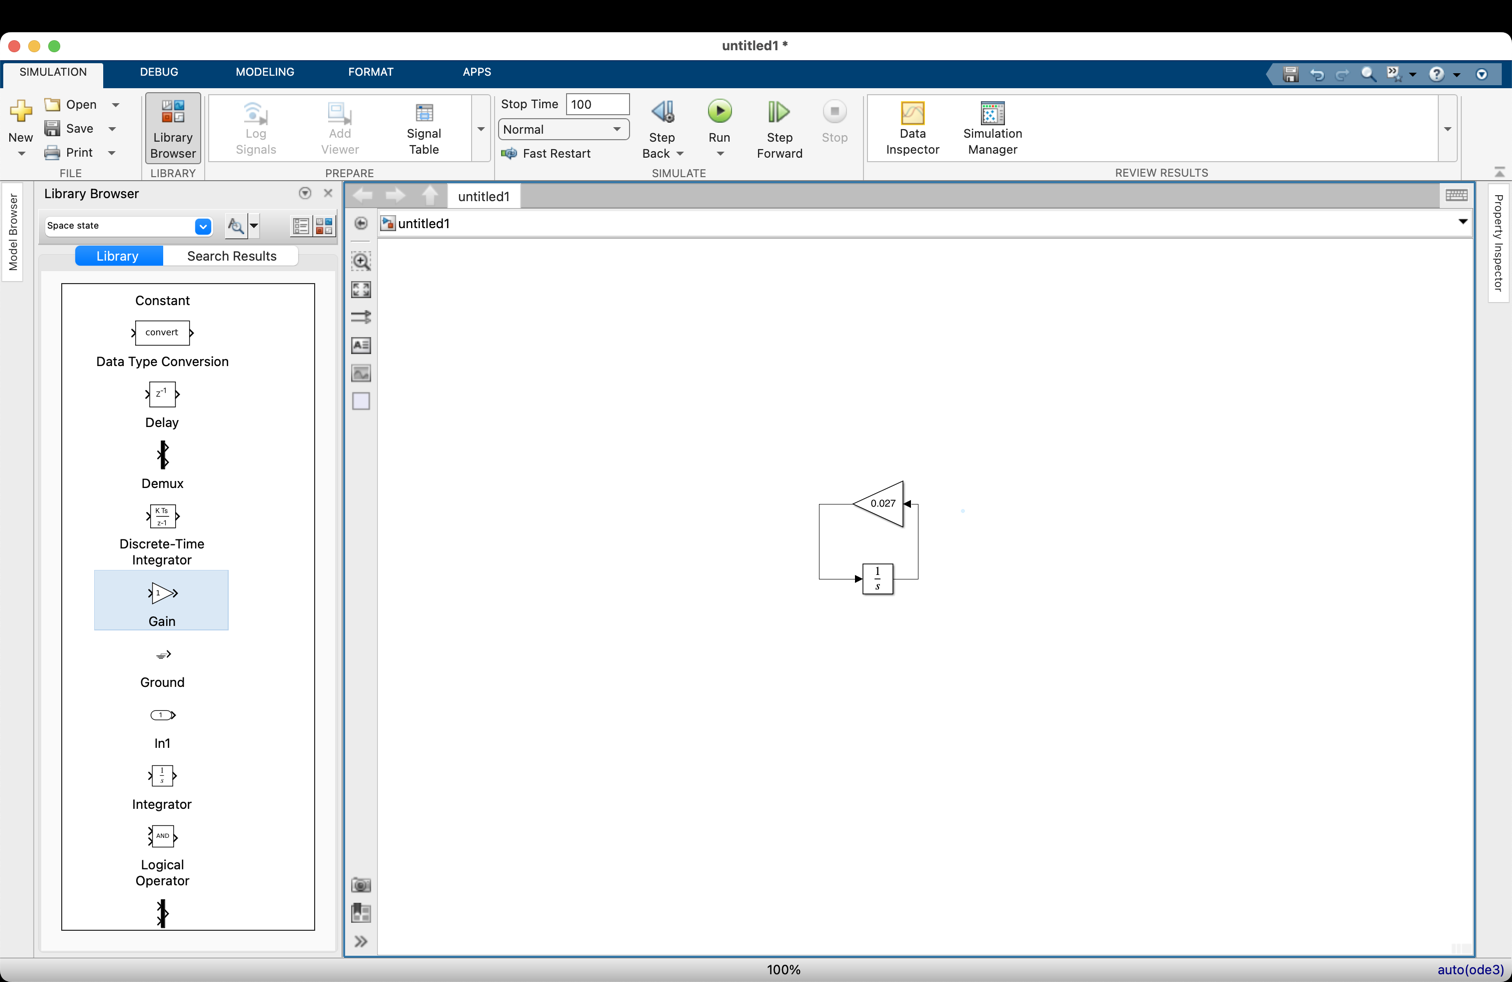
\includegraphics[width=\paperwidth]{lesson_2/images/simulink_screen_20.png}
\end{frame}

\begin{frame}{\small Initial population can be a block parameter or external constant.}
    \hspace*{-11mm}
    \only<1>{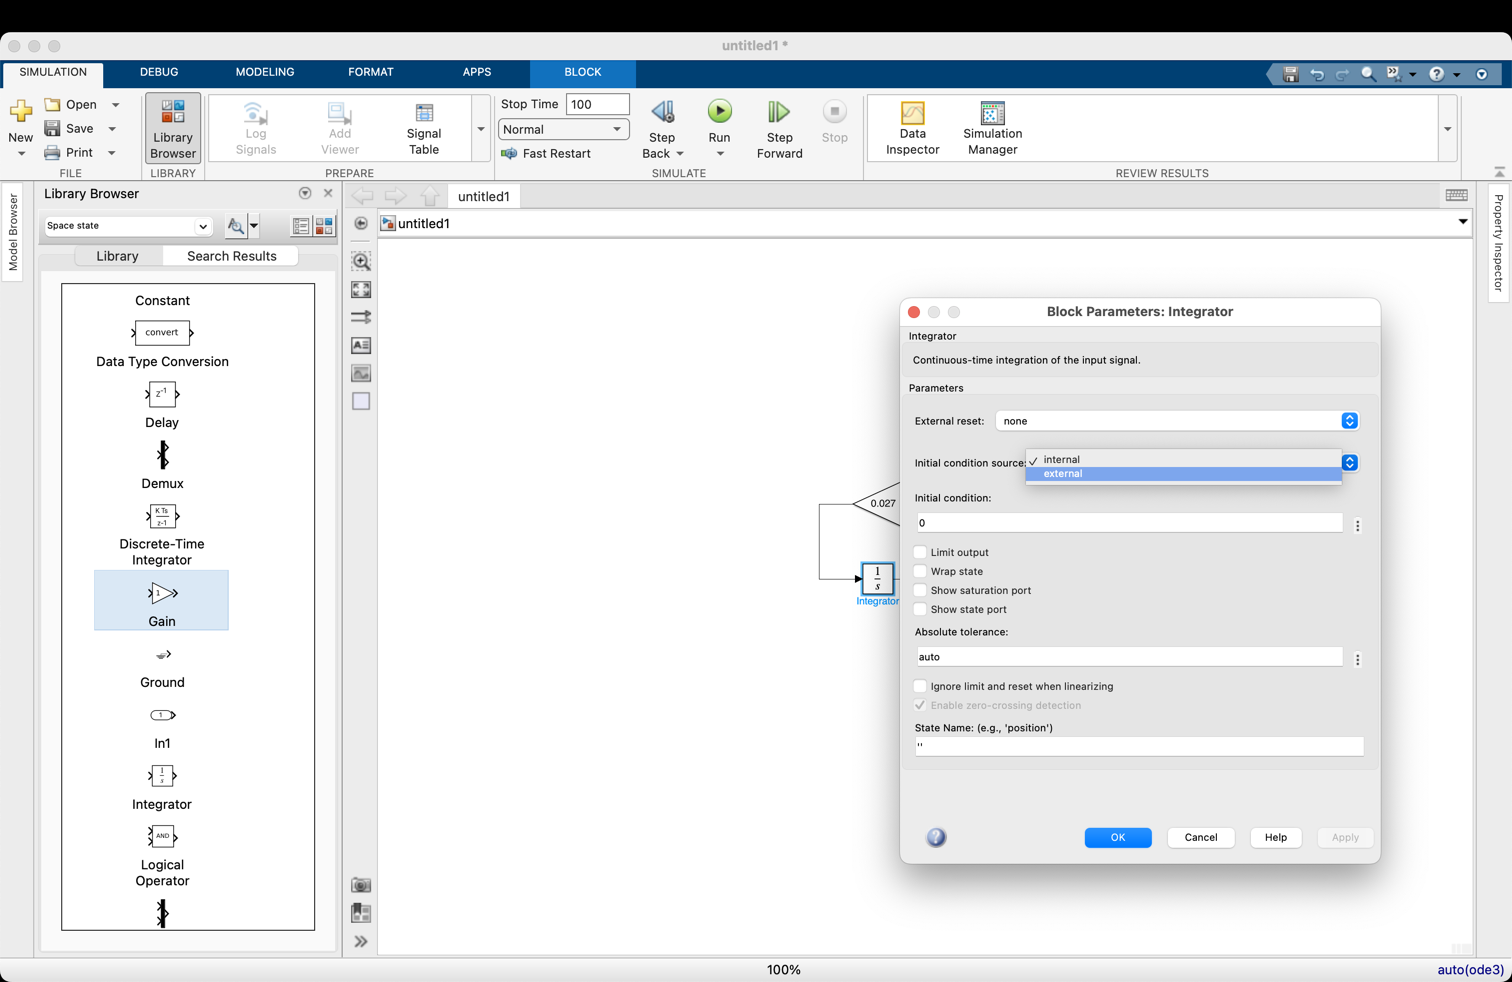
\includegraphics[width=\paperwidth]{lesson_2/images/simulink_screen_21.png}}
    \only<2>{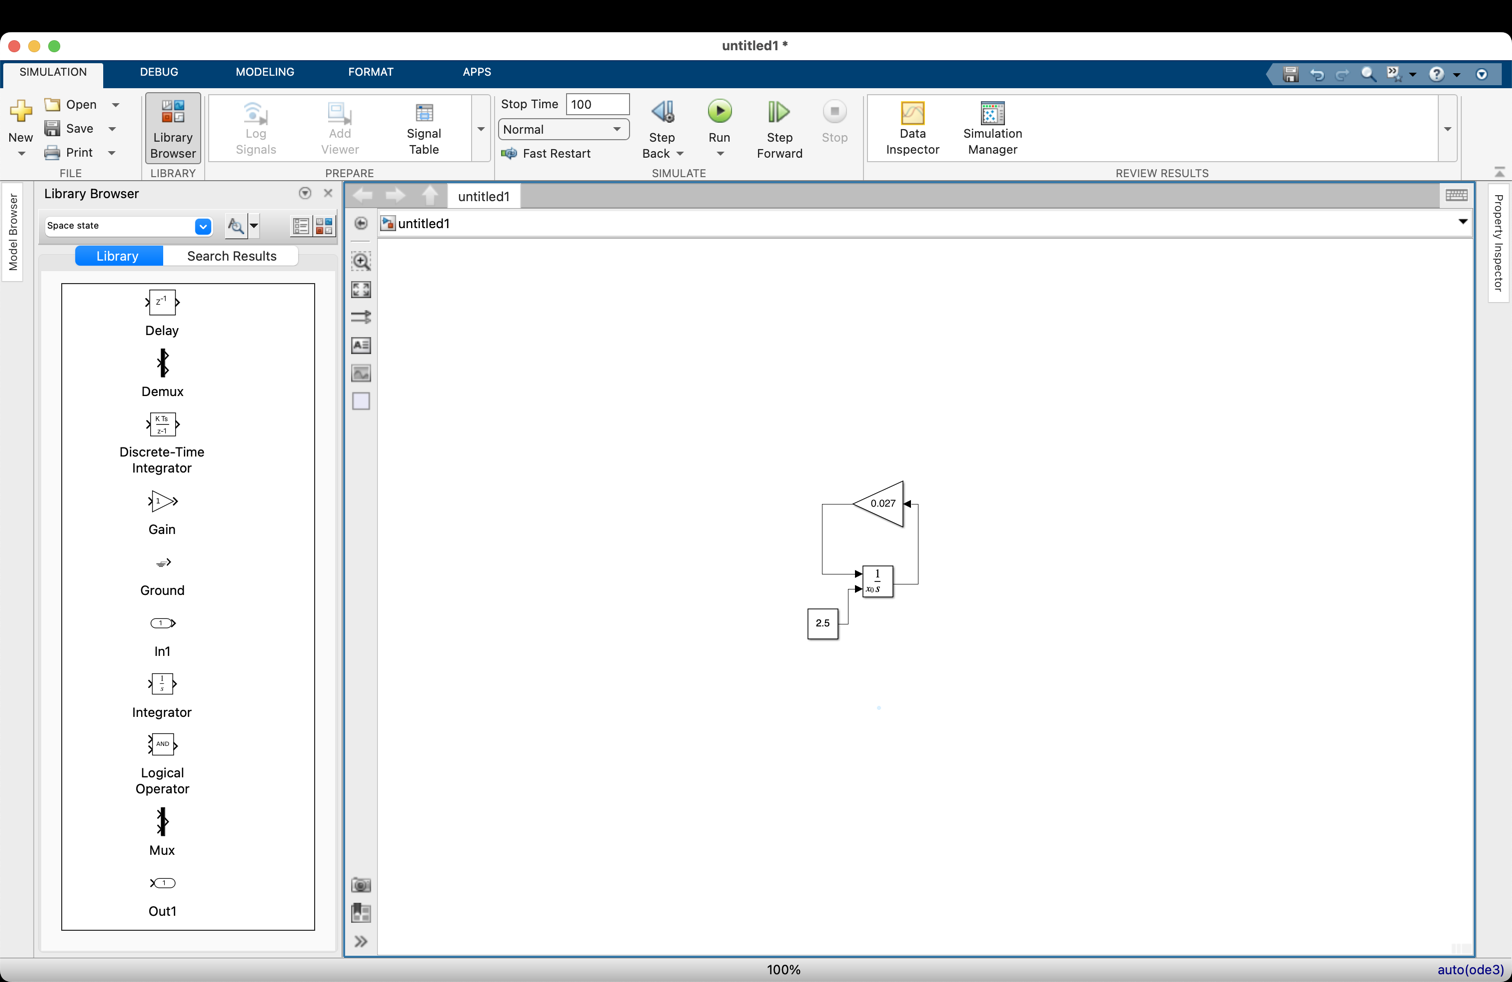
\includegraphics[width=\paperwidth]{lesson_2/images/simulink_screen_22.png}}
\end{frame}

\begin{frame}{We add display and labels}
    \hspace*{-11mm}
    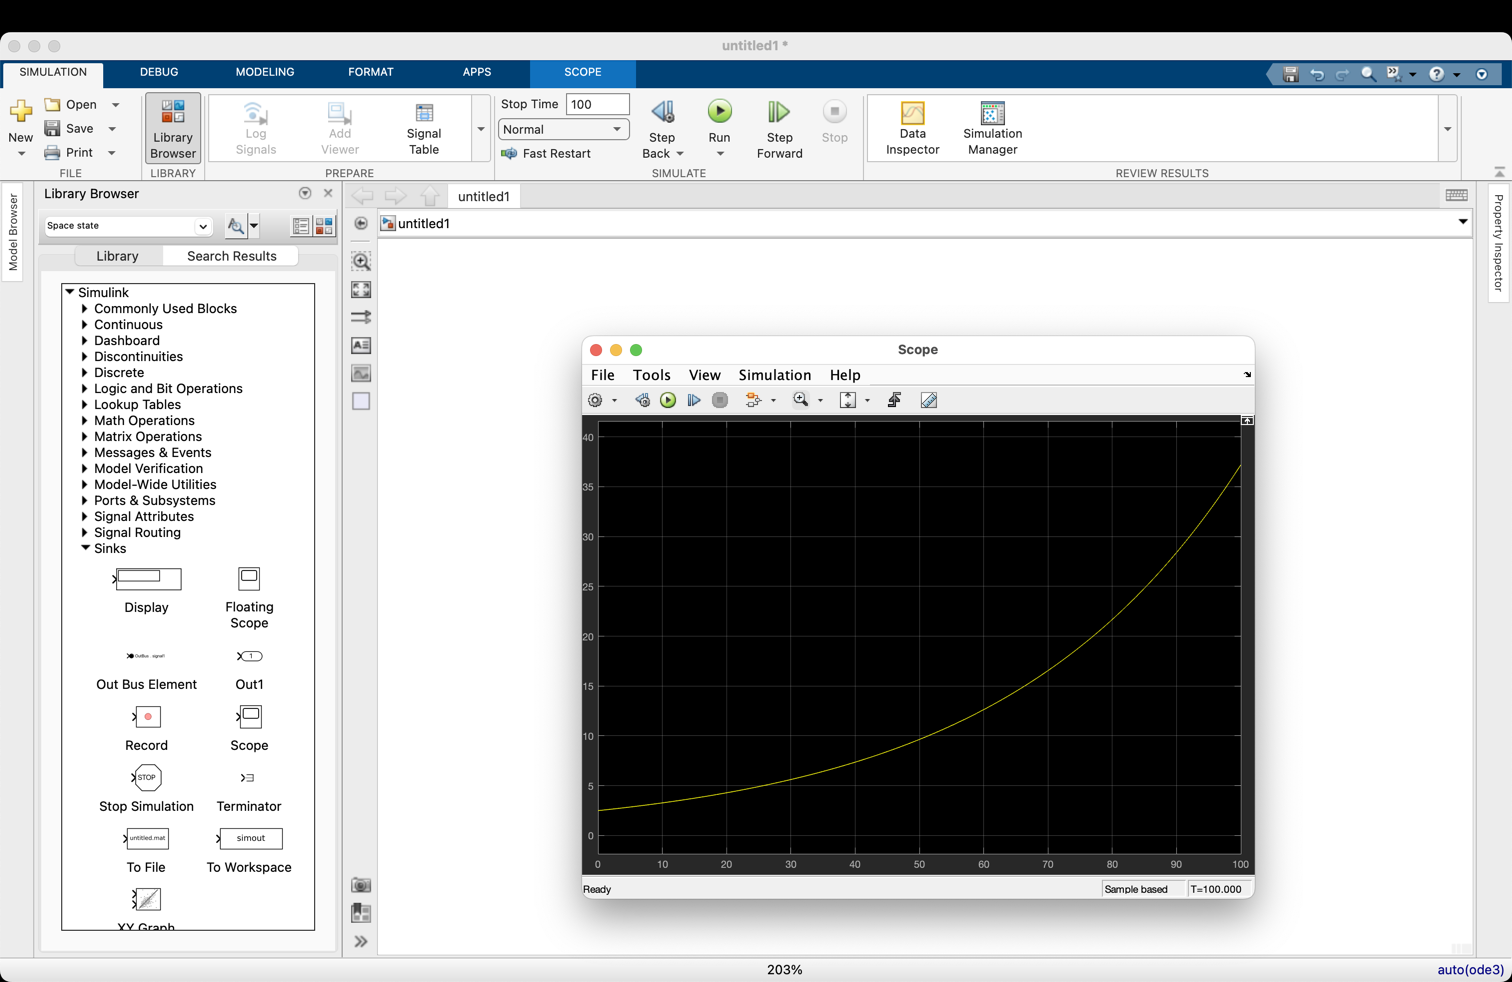
\includegraphics[width=\paperwidth]{lesson_2/images/simulink_screen_26.png}
\end{frame}

\begin{frame}{Resulting population growth}
    \hspace*{-11mm}
    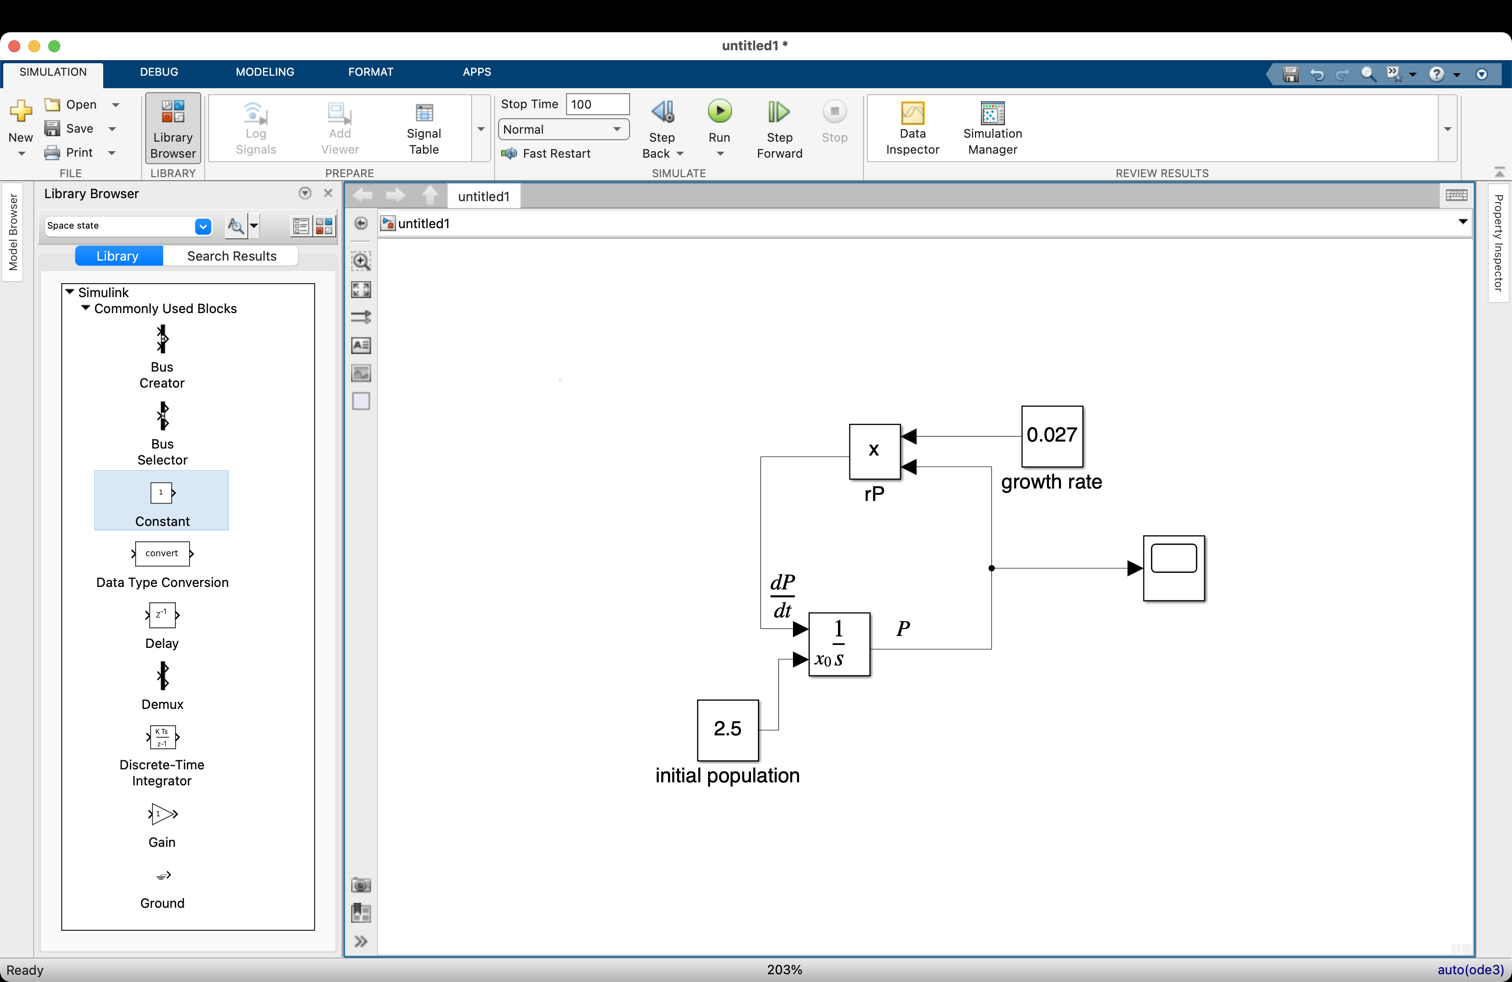
\includegraphics[width=\paperwidth]{lesson_2/images/simulink_screen_27.png}
\end{frame}

\subsection{Subsystems are equivalent of function}
\begin{frame}{Simulate for longer time}
\Large
\begin{itemize}
    \item We may create a subsystems from our diagram
    \item Subsystems are equivalent of functions in Matlab
    \item Subsystems are used to re-use and organize code
    \pause
    \item Here, we will create a subsystem from our code to run several scenarios in parallel for different growth rate
\end{itemize}
\end{frame}

\begin{frame}{We replace gain block and select relevant parts}
    \hspace*{-11mm}
    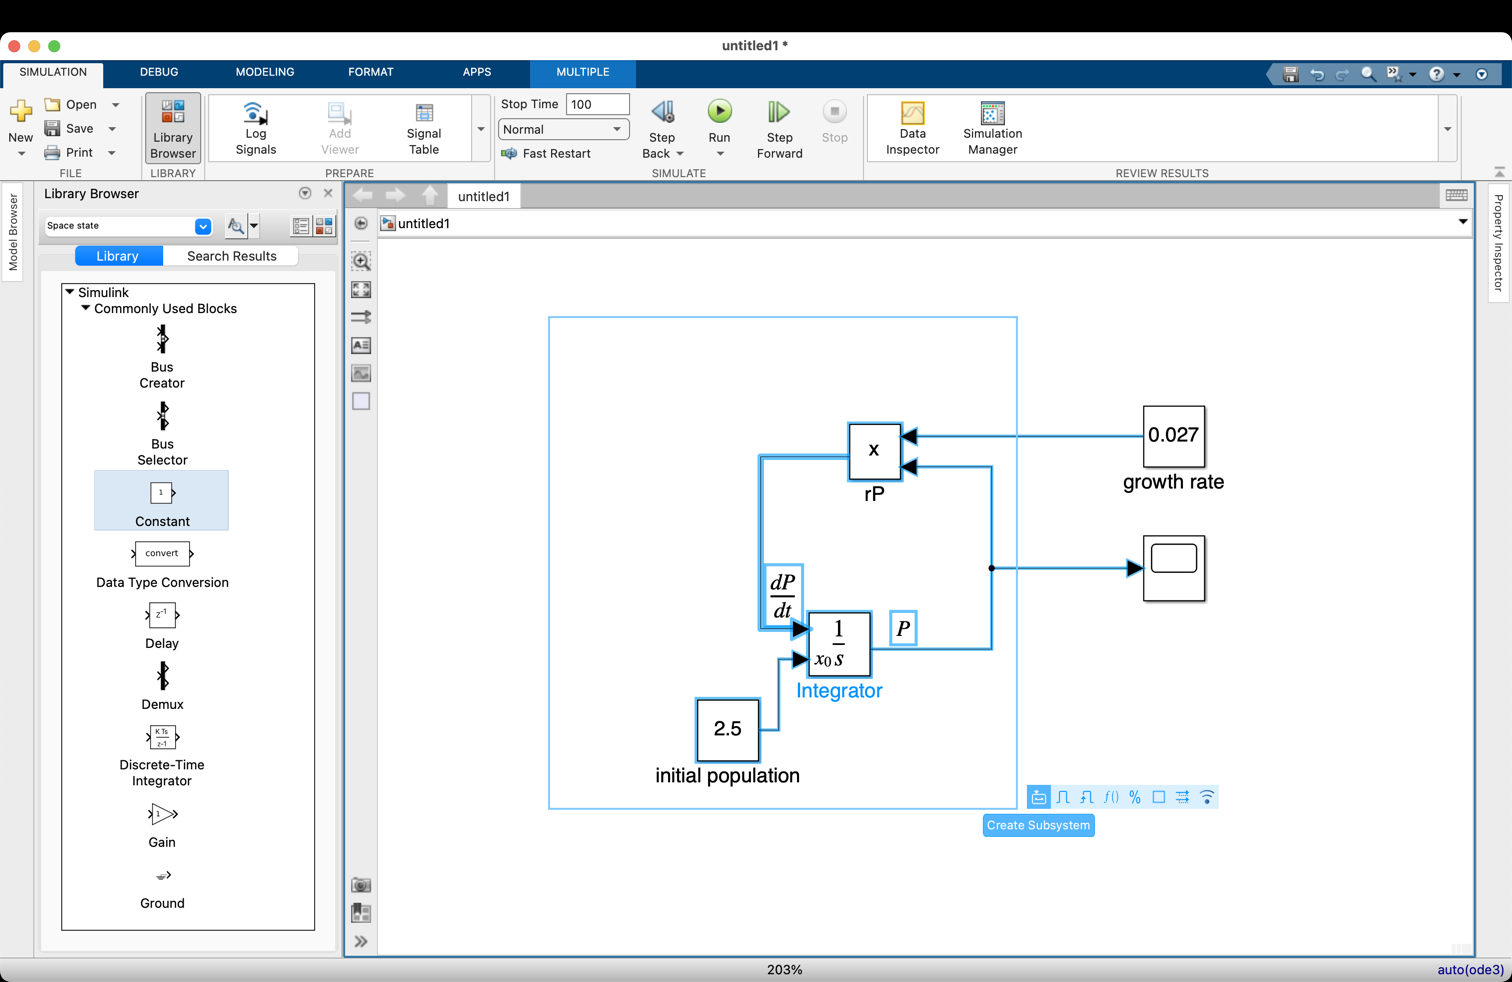
\includegraphics[width=\paperwidth]{lesson_2/images/simulink_screen_28.png}
\end{frame}

\begin{frame}{Resulting subsystem}
    \hspace*{-11mm}
    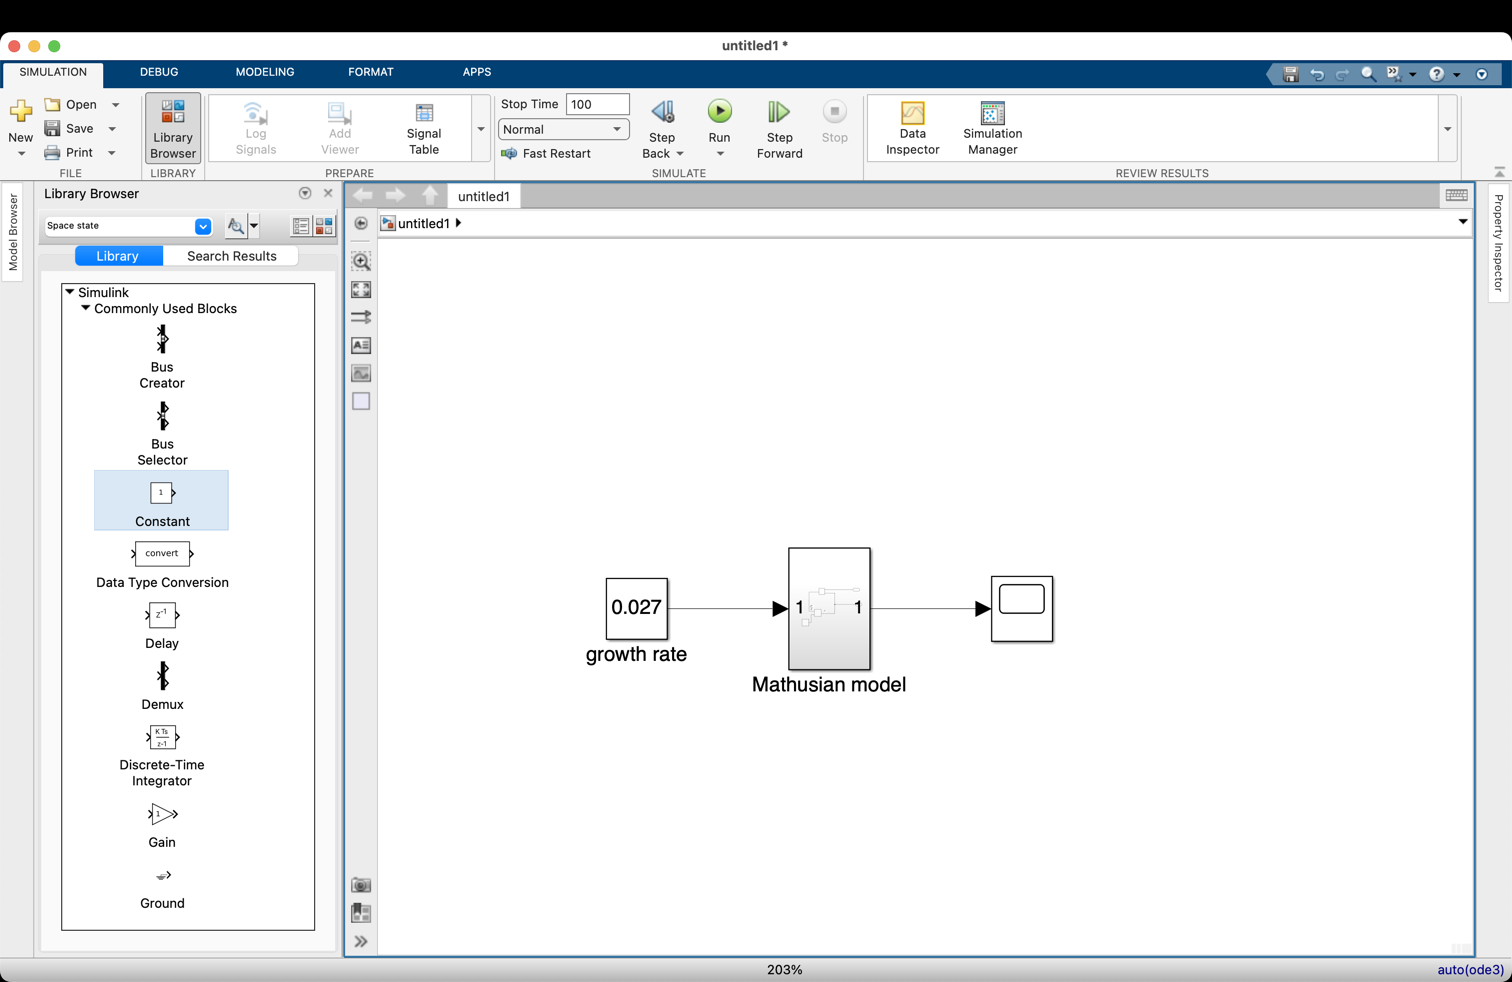
\includegraphics[width=\paperwidth]{lesson_2/images/simulink_screen_29.png}
\end{frame}

\begin{frame}{We can duplicate subsystems for parallel simulations}
    \hspace*{-11mm}
    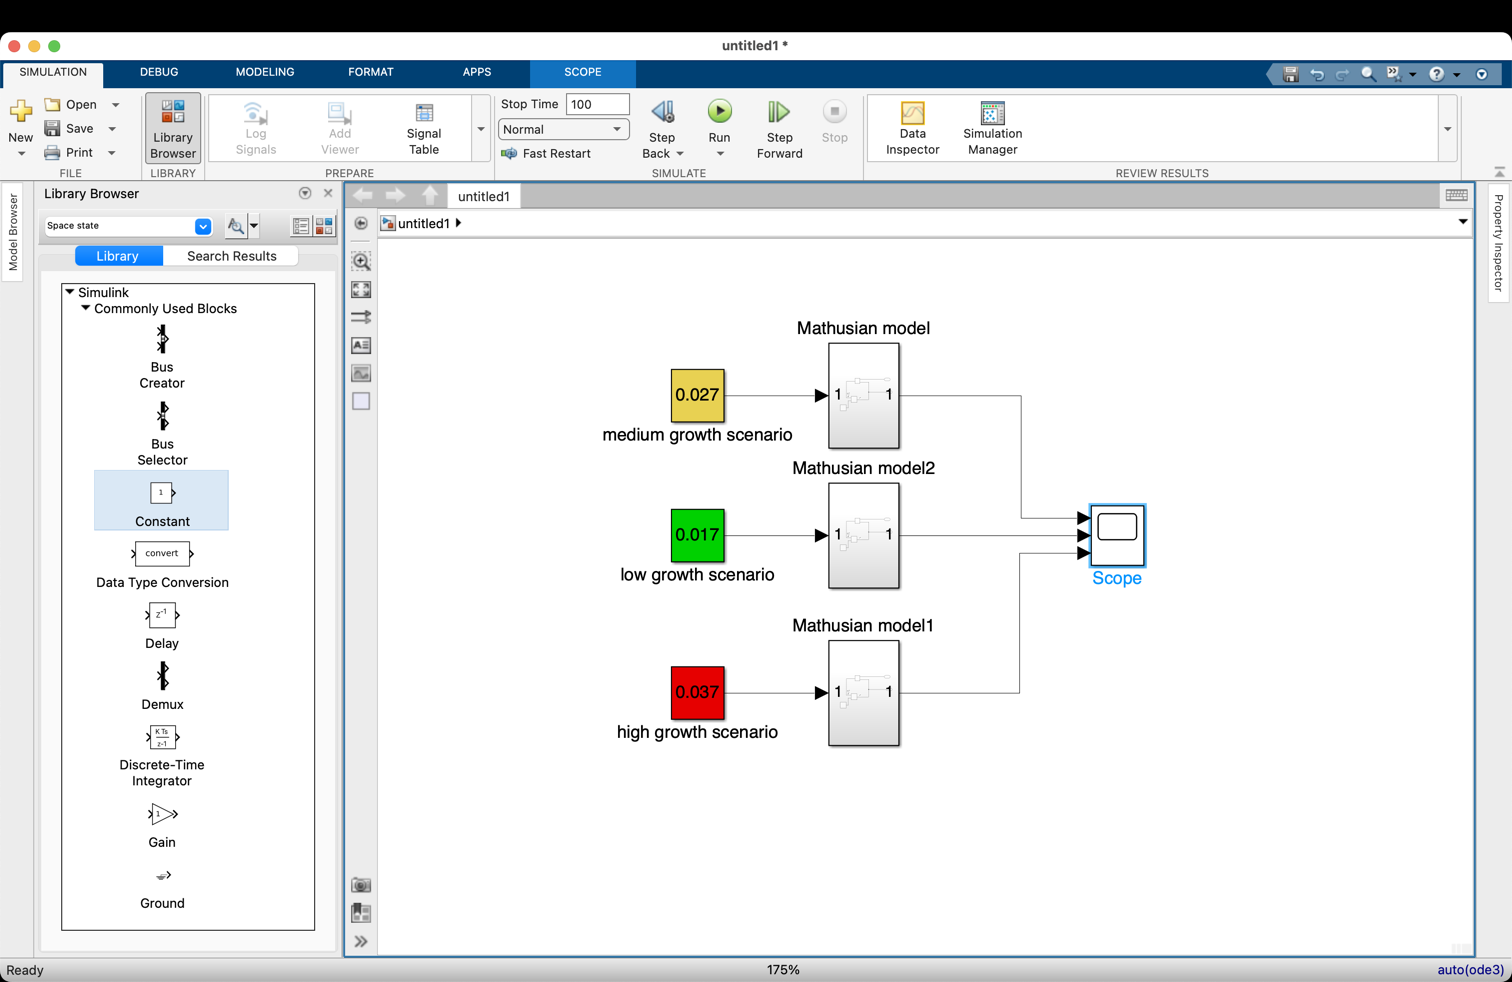
\includegraphics[width=\paperwidth]{lesson_2/images/simulink_screen_30.png}
\end{frame}

\begin{frame}{Plots can be easily adjusted}
    \hspace*{-11mm}
    \only<1>{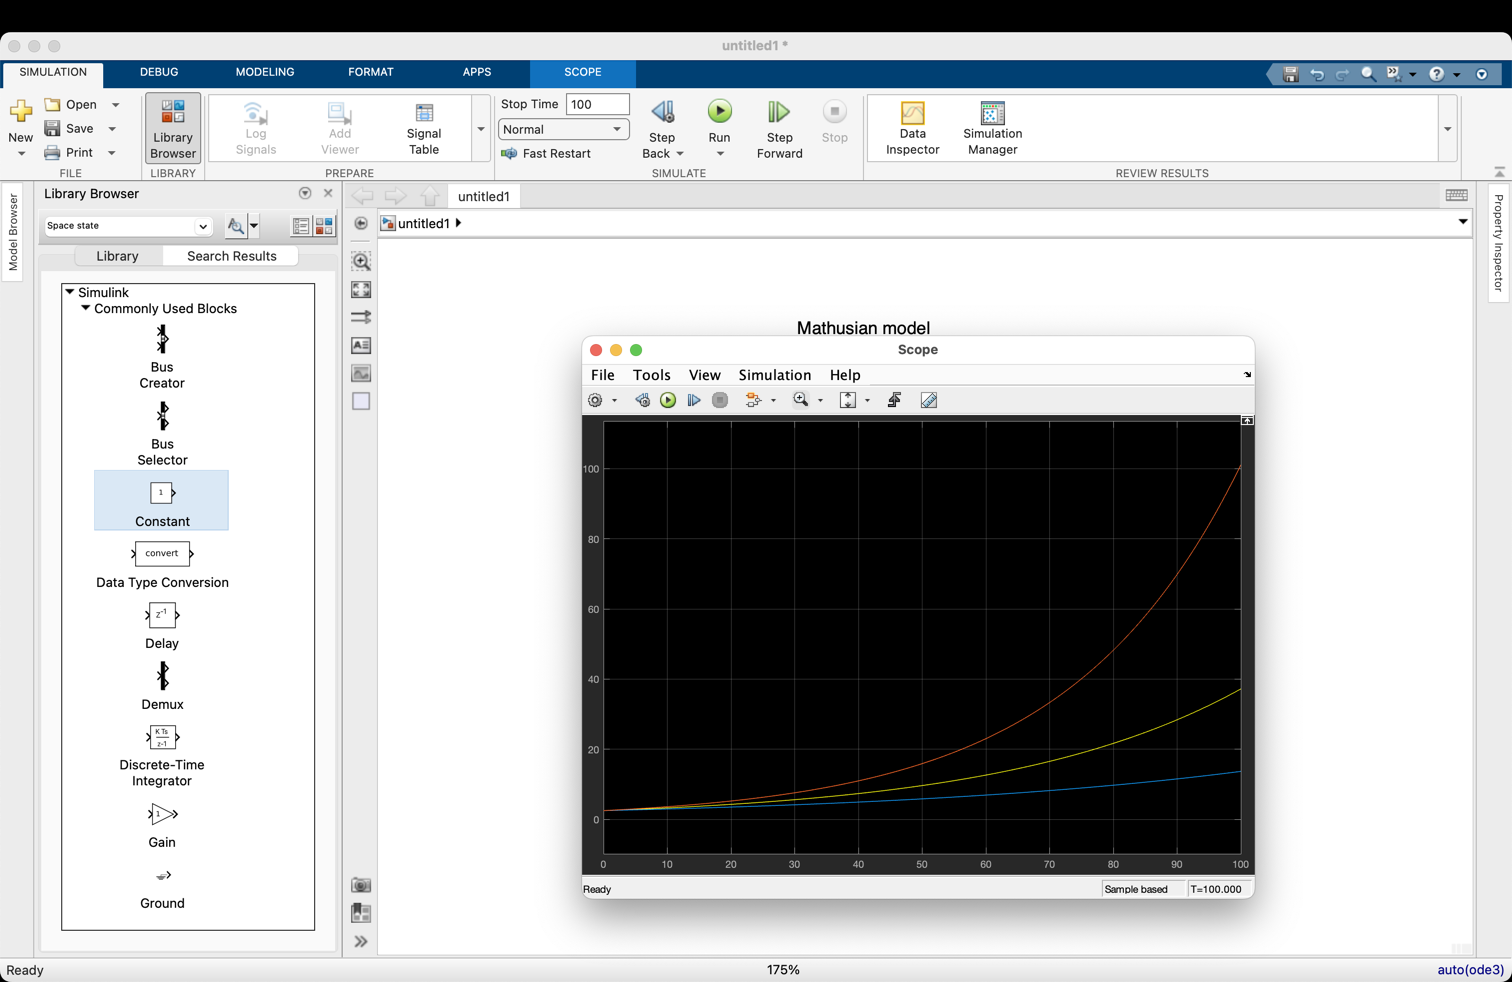
\includegraphics[width=\paperwidth]{lesson_2/images/simulink_screen_31.png}}
    \only<2>{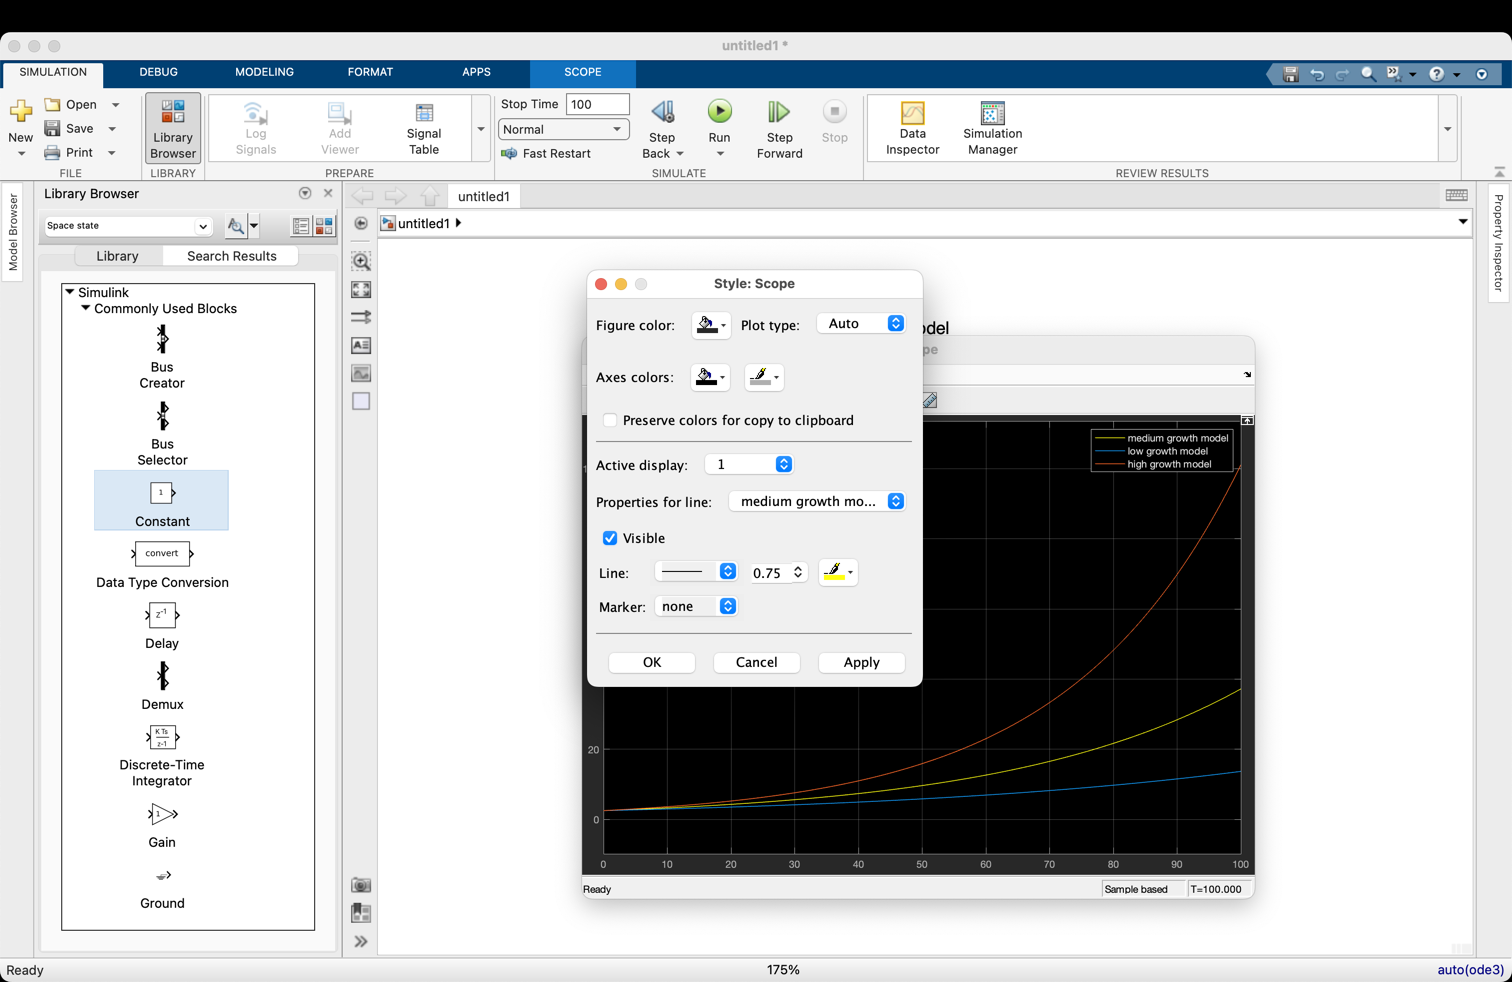
\includegraphics[width=\paperwidth]{lesson_2/images/simulink_screen_32.png}}
    \only<3>{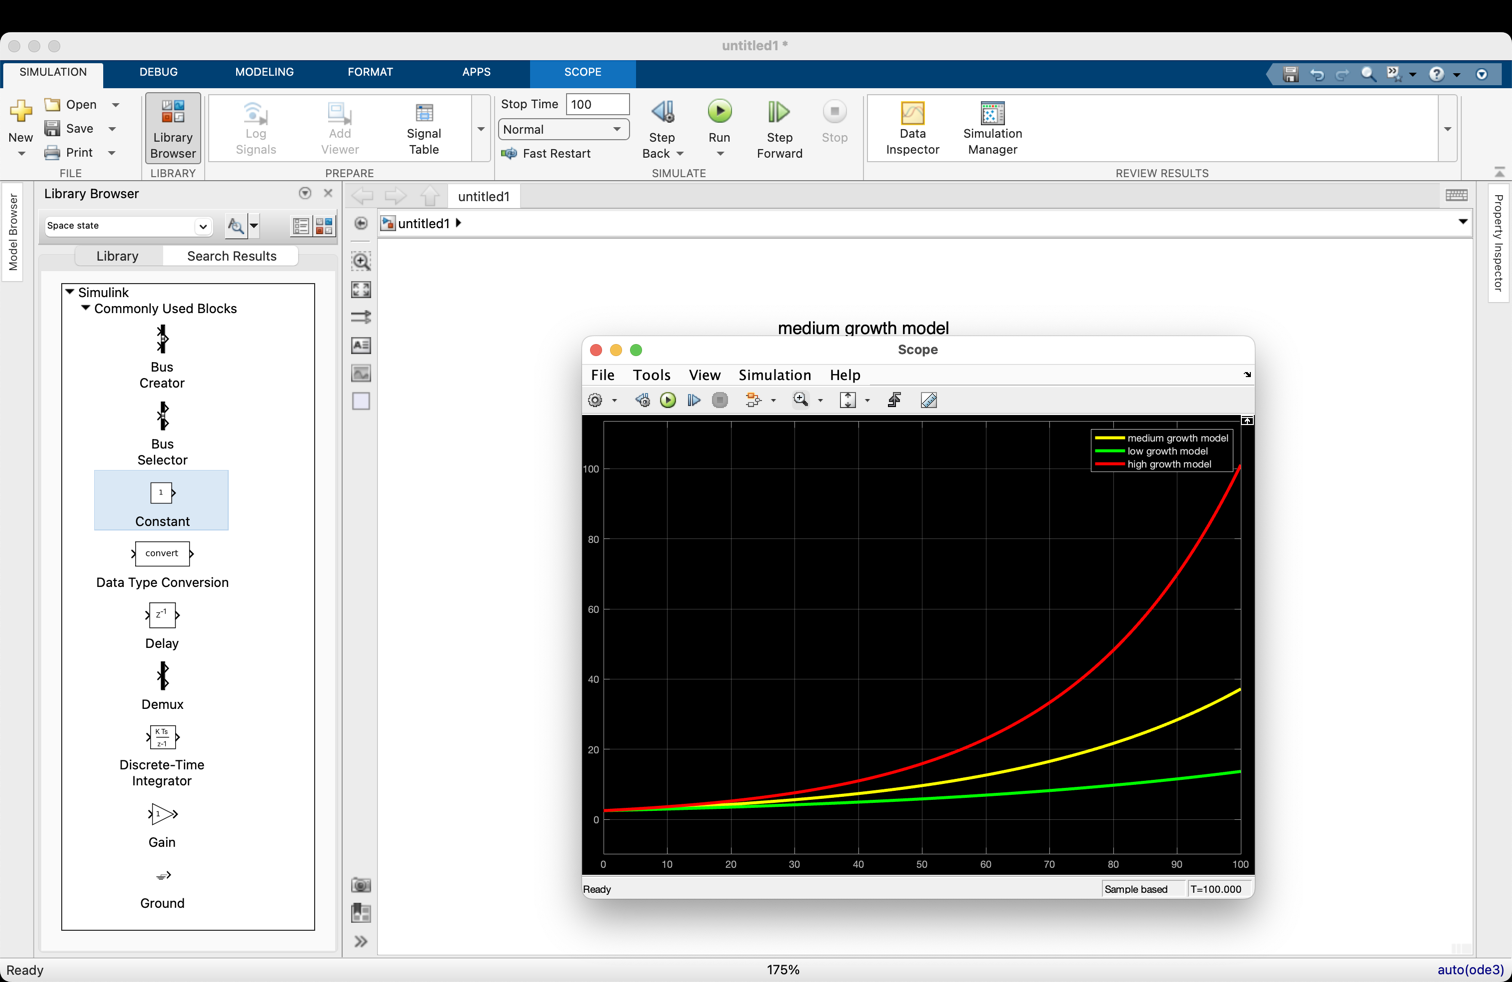
\includegraphics[width=\paperwidth]{lesson_2/images/simulink_screen_33.png}}
    \only<4>{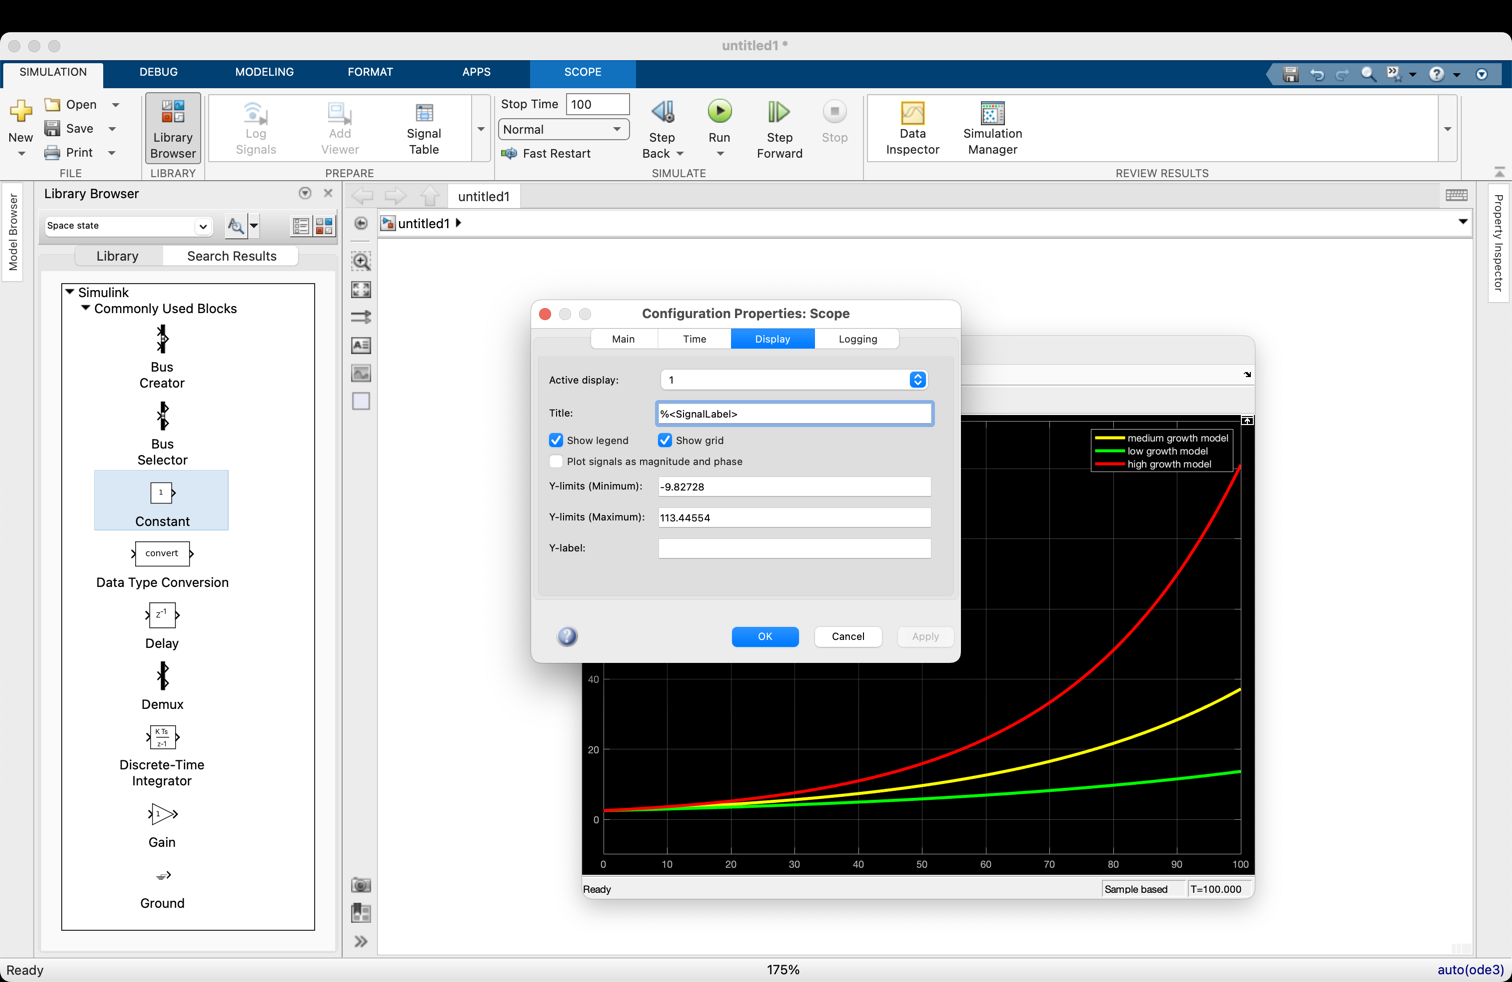
\includegraphics[width=\paperwidth]{lesson_2/images/simulink_screen_34.png}}
    \only<5>{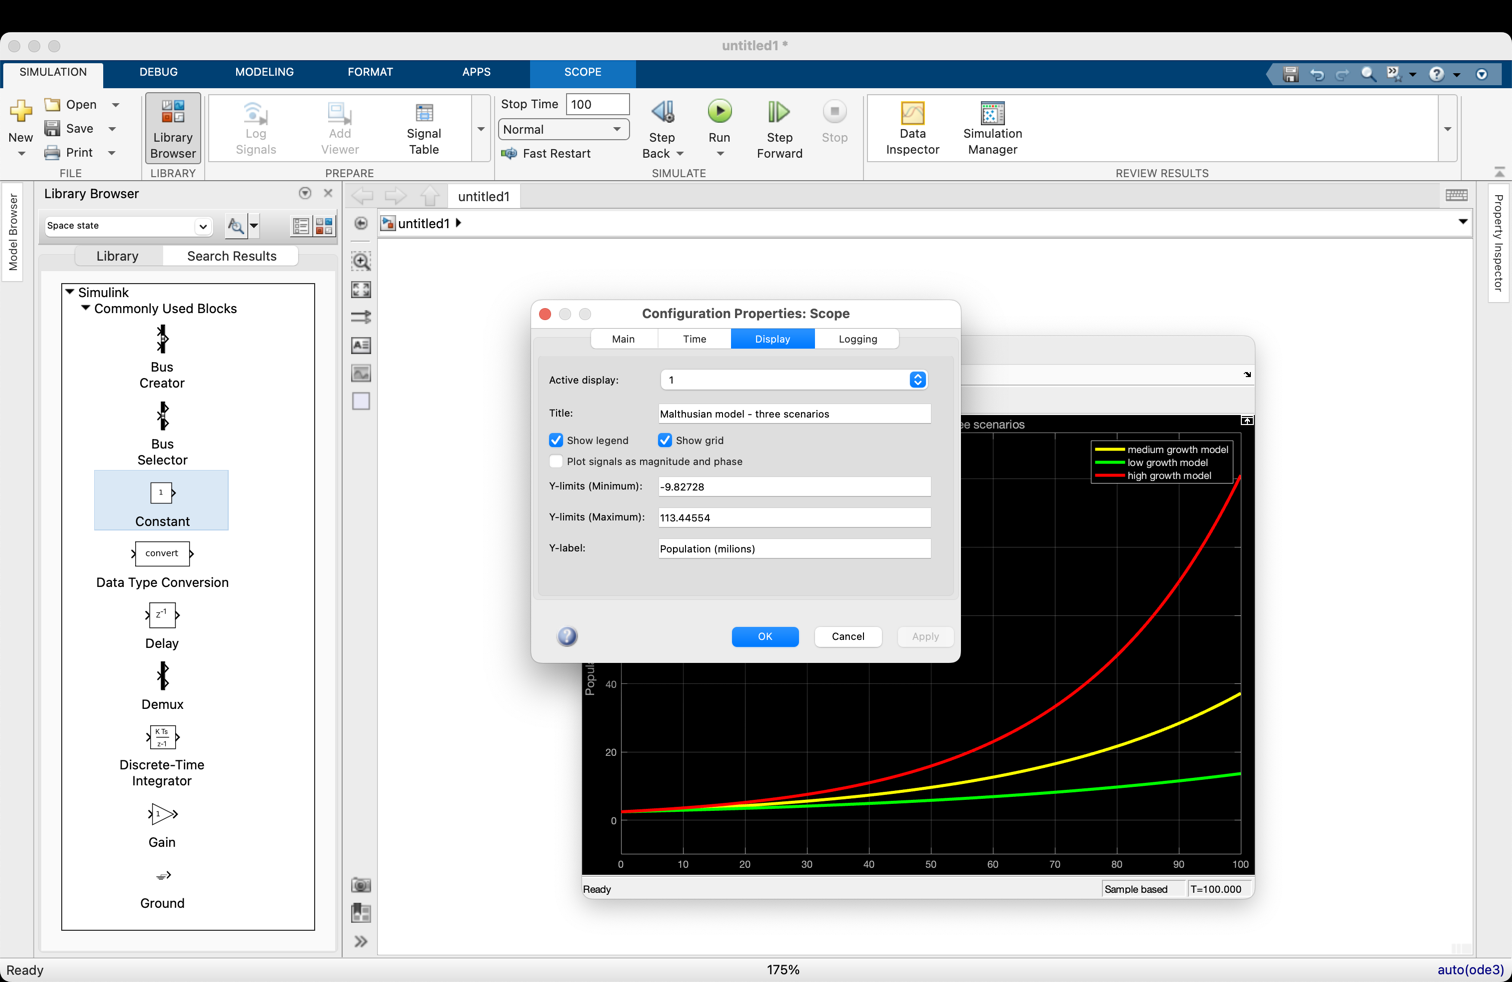
\includegraphics[width=\paperwidth]{lesson_2/images/simulink_screen_35.png}}
    \only<6>{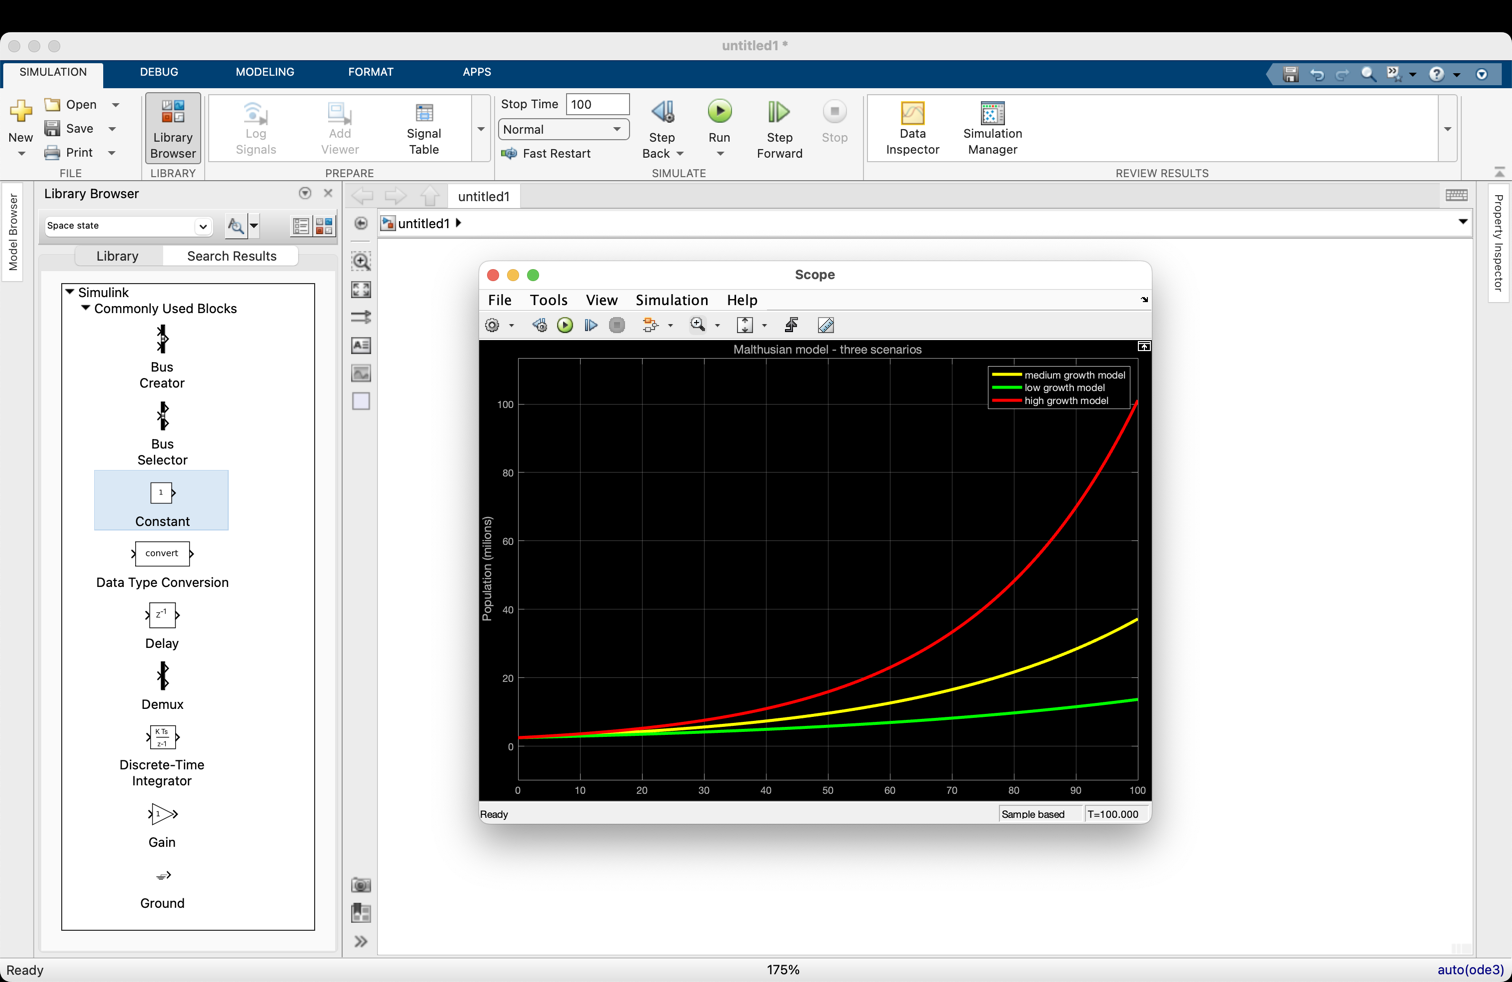
\includegraphics[width=\paperwidth]{lesson_2/images/simulink_screen_36.png}}
\end{frame}

\begin{frame}{Experiments with blocks and settings}
    \hspace*{-11mm}
    \only<1>{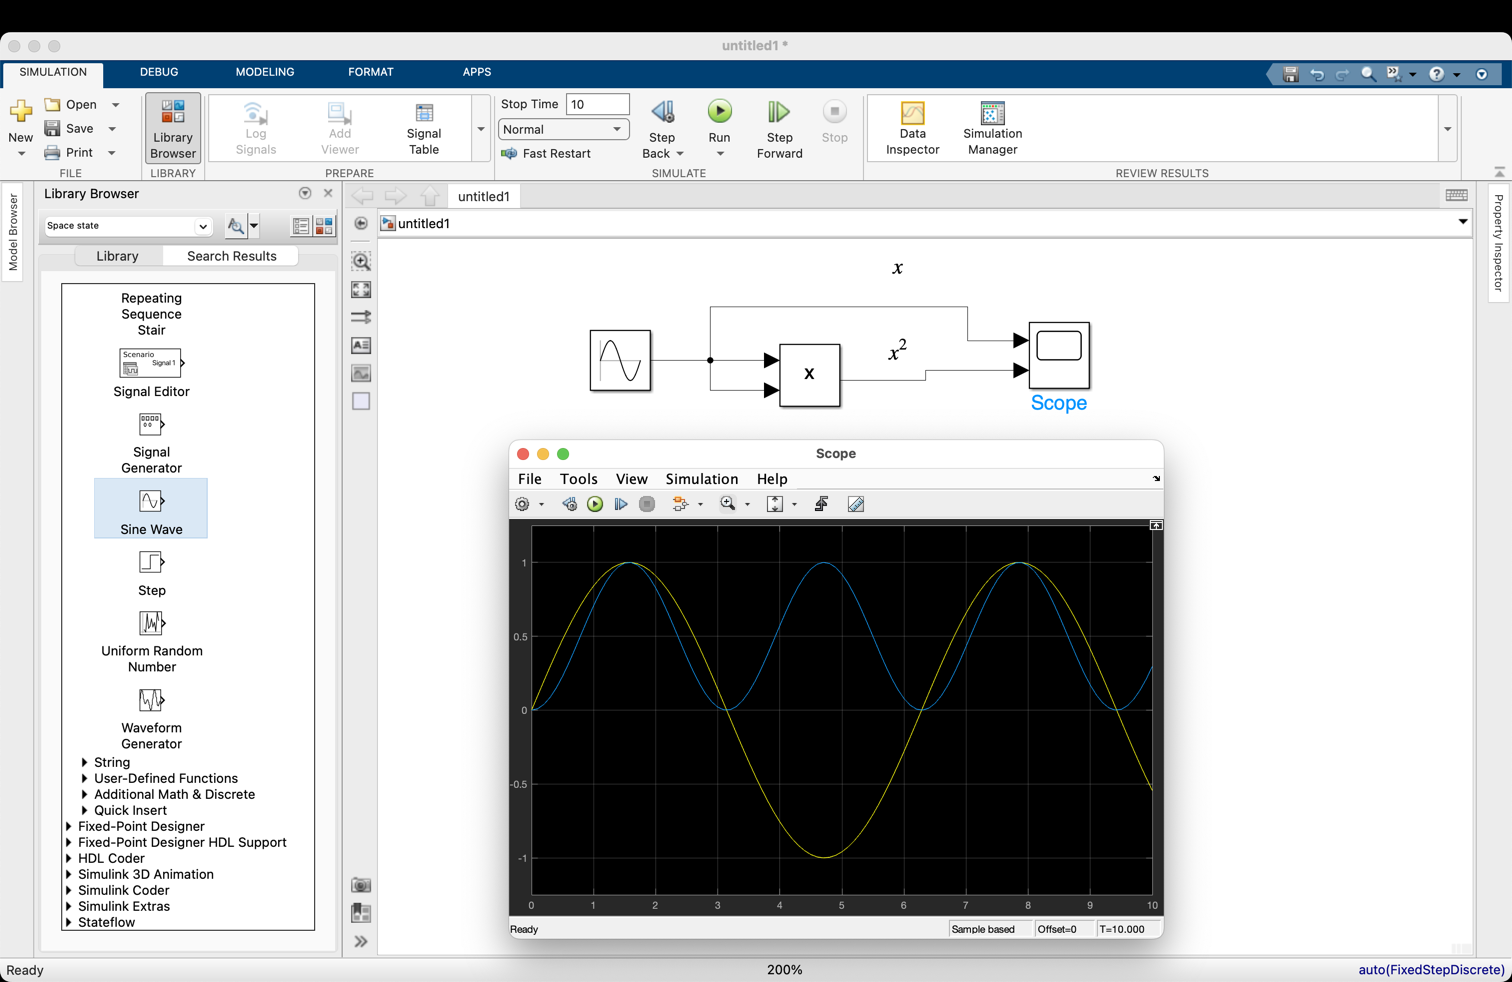
\includegraphics[width=\paperwidth]{lesson_2/images/simulink_screen_37.png}}
    \only<2>{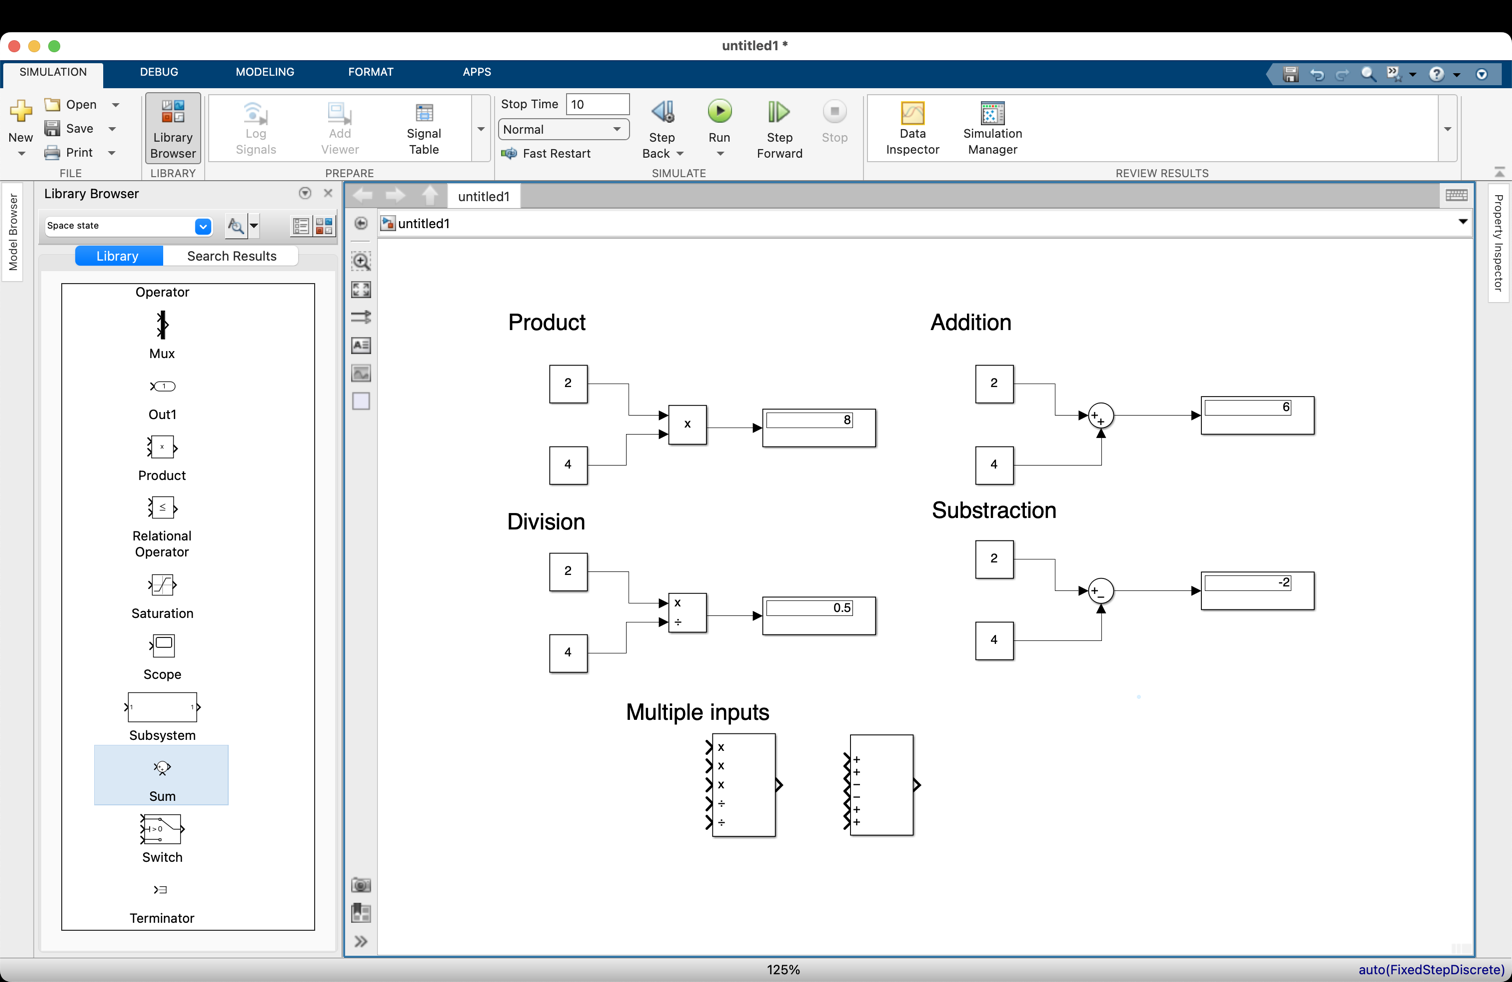
\includegraphics[width=\paperwidth]{lesson_2/images/simulink_screen_38.png}}
\end{frame}


